%%%%%%%%%%%%%%%%%%%%%%%%%%%%%%%%%%%%%%%%%%
%                                        %
% Szablon pracy dyplomowej inzynierskiej % 
%                                        %
%%%%%%%%%%%%%%%%%%%%%%%%%%%%%%%%%%%%%%%%%%



\documentclass[a4paper,twoside,12pt]{book}
\usepackage[utf8]{inputenc}                                      
\usepackage[T1]{fontenc}  
\usepackage{amsmath,amsfonts,amssymb,amsthm}
\usepackage[british,polish]{babel} 
\usepackage[utf8]{inputenc}
\usepackage{graphicx} 
\usepackage{nameref}
\usepackage{indentfirst}
\usepackage{lmodern}
\usepackage{graphicx}
\usepackage{hyperref}
\usepackage{booktabs}
\usepackage{placeins}
\usepackage{tikz}
\usepackage{pgfplots}
\usepackage{mathtools}
\usepackage{geometry}
\usepackage[page]{appendix} % toc,
\renewcommand{\appendixtocname}{Dodatki}
\renewcommand{\appendixpagename}{Dodatki}
\renewcommand{\appendixname}{Dodatek}

\usepackage{setspace}

% \usepackage{comment}
% \excludecomment{figure}
% \excludecomment{table}

% \let\endfigure\relax

\onehalfspacing


\frenchspacing

\usepackage{listings}
%\lstset{
%	language={},
%	basicstyle=\ttfamily,
%	keywordstyle=\lst@ifdisplaystyle\color{blue}\fi,
%	commentstyle=\color{gray}
%}

%%%%%%%%%%%%%%%%%%%%%%%%%%%
% listingi 
\usepackage{listings}
\lstset{%
language=C++,%
commentstyle=\textit,%
identifierstyle=\textsf,%
keywordstyle=\sffamily\bfseries, %\texttt, %
%captionpos=b,%
tabsize=3,%
frame=lines,%
numbers=left,%
numberstyle=\tiny,%
numbersep=5pt,%
breaklines=true,%
morekeywords={descriptor_gaussian,descriptor,partition,fcm_possibilistic,dataset,my_exception,exception,std,vector},%
escapeinside={@*}{*@},%
%texcl=true, % wylacza tryb verbatim w komentarzach jednolinijkowych
}
%%%%%%%%%%%%%%%%%%%%%%%%%%%%%%%%%%%%


%%%%%%%%%

%%%% TODO LIST GENERATOR %%%%%%%%%

%\usepackage{tikz}
%\usepackage{manfnt}   % dangerous sign 
\usepackage{color}
\definecolor{brickred}      {cmyk}{0   , 0.89, 0.94, 0.28}

\makeatletter \newcommand \kslistofremarks{\section*{Uwagi} \@starttoc{rks}}
  \newcommand\l@uwagas[2]
    {\par\noindent \textbf{#2:} %\parbox{10cm}
{#1}\par} \makeatother


\newcommand{\ksremark}[1]{%
{%\marginpar{\textdbend}
{\color{brickred}{[#1]}}}%
\addcontentsline{rks}{uwagas}{\protect{#1}}%
}

\newcommand{\comma}{\ksremark{przecinek}}
\newcommand{\nocomma}{\ksremark{bez przecinka}}
\newcommand{\styl}{\ksremark{styl}}
\newcommand{\ortografia}{\ksremark{ortografia}}
\newcommand{\fleksja}{\ksremark{fleksja}}
\newcommand{\pauza}{\ksremark{pauza `--', nie dywiz `-'}}
\newcommand{\kolokwializm}{\ksremark{kolokwializm}}

%%%%%%%%%%%%%% END OF TODO LIST GENERATOR %%%%%%%%%%%

%%%%%%%%%%%% ZYWA PAGINA %%%%%%%%%%%%%%%
% brak kapitalizacji zywej paginy
\usepackage{fancyhdr}
\pagestyle{fancy}
\fancyhf{}
\fancyhead[LO]{\nouppercase{\it\rightmark}}
\fancyhead[RE]{\nouppercase{\it\leftmark}}
\fancyhead[LE,RO]{\it\thepage}


\fancypagestyle{tylkoNumeryStron}{%
   \fancyhf{} 
   \fancyhead[LE,RO]{\it\thepage}
}

\fancypagestyle{NumeryStronNazwyRozdzialow}{%
   \fancyhf{} 
   \fancyhead[LO]{\nouppercase{\it\rightmark}}
   \fancyhead[RE]{\nouppercase{\it\leftmark}}
   \fancyhead[LE,RO]{\it\thepage}
}


%%%%%%%%%%%%% OBCE WTRETY  
\newcommand{\obcy}[1]{\emph{#1}}
\newcommand{\ang}[1]{{\selectlanguage{british}\obcy{#1}}}
%%%%%%%%%%%%%%%%%%%%%%%%%%%%%

% polskie oznaczenia funkcji matematycznych
\renewcommand{\tan}{\operatorname {tg}}
\renewcommand{\log}{\operatorname {lg}}

% jeszcze jakies drobiazgi

\newcounter{stronyPozaNumeracja}

\newcommand{\hcancel}[1]{%
    \tikz[baseline=(tocancel.base)]{
        \node[inner sep=0pt,outer sep=0pt] (tocancel) {#1};
        \draw[red] (tocancel.south west) -- (tocancel.north east);
    }%
}%

\newcommand{\miesiac}{%
  \ifcase\the\month
  \or styczeń% 1
  \or luty% 2
  \or marzec% 3
  \or kwiecień% 4
  \or maj% 5
  \or czerwiec% 6
  \or lipiec% 7
  \or sierpień% 8
  \or wrzesień% 9
  \or październik% 10
  \or listopad% 11
  \or grudzień% 12
  \fi}


%%%%%%%%%%%%%%%%%%%%%%%%%%%%%%%%%%%%%%%%%%%%%%
% Helvetica font macros for the title page:
\newcommand{\headerfont}{\fontfamily{phv}\fontsize{18}{18}\bfseries\scshape\selectfont}
\newcommand{\titlefont}{\fontfamily{phv}\fontsize{18}{18}\selectfont}
\newcommand{\otherfont}{\fontfamily{phv}\fontsize{14}{14}\selectfont}

%%%%%%%%%%%%%%%%%%%%%%%%%%%%%%%%%%%%%%%%%%%%%%
%%%%%%%%%%%%%%%%%%%%%%%%%%%%%%%%%%%%%%%%%%%%%%
%%%%%%%%%%%%%%%%%%%%%%%%%%%%%%%%%%%%%%%%%%%%%%
%%%%%%%%%%%%%%%%%%%%%%%%%%%%%%%%%%%%%%%%%%%%%%
%%%%%%%%%%%%%%%%%%%%%%%%%%%%%%%%%%%%%%%%%%%%%%
%%%%%%%%%%%%%%%%%%%%%%%%%%%%%%%%%%%%%%%%%%%%%%
%%%%%%%%%%%%%%%%%%%%%%%%%%%%%%%%%%%%%%%%%%%%%%


\newcommand{\autor}{Bartłomiej Gładys}
\newcommand{\promotor}{dr inż. Jakub Nalepa}
\newcommand{\tytul}{
Analiza zachowań ludzkich na bazie aktywności rejestrowanych 
w~aplikacjach mobilnych z wykorzystaniem metod uczenia maszynowego
}
\newcommand{\polsl}{Politechnika Śląska}
\newcommand{\wydzial}{Wydział Automatyki, Elektroniki i Informatyki}


\begin{document}
%\kslistofremarks 
	
%%%%%%%%%%%%%%%%%%  STRONA TYTULOWA %%%%%%%%%%%%%%%%%%%
\pagestyle{empty}
{
	\newgeometry{top=2.5cm,%
	             bottom=2.5cm,%
	             left=3cm,
	             right=2.5cm}
	\sffamily
	\rule{0cm}{0cm}
	
	\begin{center}
	
\includegraphics[width=29mm]{polsl}
	\end{center} 
	\vspace{1cm}
	\begin{center}
	\headerfont \polsl
	\end{center}
	\begin{center}
	\headerfont \wydzial
	\end{center}
	\vfill
	\begin{center}
	\titlefont Praca dyplomowa inżynierska
	\end{center}
	\vfill
	
	\begin{center}
	\otherfont \tytul\par
	\end{center}
	
	\vfill
	
	\vfill
	 
	\noindent\vbox
	{
		\hbox{\otherfont autor: \autor}
		\vspace{12pt}
		\hbox{\otherfont kierujący pracą: \promotor}
		\vspace{12pt}  % zakomentuj, jezeli nie ma konsultanta
% 		\hbox{\otherfont konsultant: \konsultant} % zakomentuj, jezeli nie ma konsultanta
	}
	\vfill 
 
   \begin{center}
   \otherfont Gliwice,  \miesiac\ \the\year
   \end{center}	
	\restoregeometry
}
  

\cleardoublepage
 

\rmfamily
\normalfont

%%%%%%%%%%%%%%%%%%%%% oswiadczenie o udostępnianiu pracy dyplomowej %%%%%%%%%%%%%%%%%%%
\cleardoublepage

\begin{flushright}
załącznik nr 2 do zarz. nr 97/08/09 
\end{flushright}

\vfill  

\begin{center}
\Large\bfseries Oświadczenie
\end{center}

\vfill

Wyrażam  zgodę / Nie wyrażam zgody*  na  udostępnienie  mojej  pracy  dyplomowej / rozprawy doktorskiej*.

\vfill

Gliwice, dnia \today

\vfill

\rule{0.5\textwidth}{0cm}\dotfill 

\rule{0.5\textwidth}{0cm}
\begin{minipage}{0.45\textwidth}
{\begin{center}(podpis)\end{center}}
\end{minipage} 

\vfill

\rule{0.5\textwidth}{0cm}\dotfill 

\rule{0.5\textwidth}{0cm}
\begin{minipage}{0.45\textwidth}
{\begin{center}\rule{0mm}{5mm}(poświadczenie wiarygodności podpisu przez Dziekanat)\end{center}}
\end{minipage}


\vfill

* podkreślić właściwe

 


%%%%%%%%%%%%%%%%%%%%% oswiadczenie promotora o spełnieniu wymagań formalnych %%%%%%%%%%%%%%%%%%%
\cleardoublepage

\rule{1cm}{0cm}

\vfill  

\begin{center}
\Large\bfseries Oświadczenie promotora
\end{center}

\vfill

Oświadczam, że praca „\tytul” spełnia wymagania formalne pracy dyplomowej inżynierskiej.

\vfill



\vfill

Gliwice, dnia \today

\rule{0.5\textwidth}{0cm}\dotfill 

\rule{0.5\textwidth}{0cm}
\begin{minipage}{0.45\textwidth}
{\begin{center}(podpis promotora)\end{center}}
\end{minipage} 

\vfill

 

\cleardoublepage


%%%%%%%%%%%%%%%%%% SPIS TRESCI %%%%%%%%%%%%%%%%%%%%%%
\pagenumbering{Roman}
\pagestyle{tylkoNumeryStron}
\tableofcontents

%%%%%%%%%%%%%%%%%%%%%%%%%%%%%%%%%%%%%%%%%%%%%%%%%%%%%
\setcounter{stronyPozaNumeracja}{\value{page}}
\mainmatter
\pagestyle{NumeryStronNazwyRozdzialow}

%%%%%%%%%%%%%% wlasciwa tresc pracy %%%%%%%%%%%%%%%%%

\chapter{Wstęp i cel pracy}
\label{chap:intro}

Ludzie często nie wiedzą dlaczego ich samopoczucie bywa gorsze lub lepsze. Niewątpliwie można stwierdzić, że wpływa na to wiele czynników tj. stres, bieżące wydarzenia, czy też uwarunkowania społeczne. Niniejszy projekt inżynierski skupia się na czynniku technologicznym, który otacza nas wszystkich często nie pozwalając na moment skupienia, czy też wyciszenia. Praca ma więc za zadanie pomóc użytkownikowi w odszukaniu nawyków związanych z używaniem aplikacji mobilnych, które wpływają na niego negatywnie, oraz uświadomić jak często oraz w jakich porach dnia dane aplikacje są przez niego uruchamiane.     

Celem pracy jest implementacja narzędzia, które pozwoli zbierać dane od użytkowników i klasyfikować ich aktywności jako takie, które mają pozytywny wpływ, oraz takie które wpływają na niego w niepożądany sposób. Dzięki takiemu narzędziu osoba, która będzie je posiadać może zniwelować czas jaki poświęca na aplikacje, które podświadomie są przez nią źle odbierane. Może także dowiedzieć się w jaki sposób wpływa na nią spędzanie czasu podczas korzystania z technologi mobilnych w trakcie pewnego etapu dnia.
Zakres pracy obejmuje stworzenie aplikacji mobilnej która będzie w stanie pobierać z urządzenia dane historyczne wszystkich aktywności oraz udostępniać użytkownikowi opcje oceny jego samopoczucia oraz produktywności w ciągu dnia. Analiza wpływu aplikacji i korelacja między nimi, a czasem w którym użytkownik z nich korzysta, będzie odbywać się wewnątrz zaimplementowanego systemu w ramach pracy dyplomowej. Kolejnym punktem objętym w pracy jest stworzenie serwisów (elementów mogących działać w separacji i komunikować się między sobą przez określony protokół), które będą w stanie zbierać uzyskane dane z wielu urządzeń mobilnych, przekształcać je do formatu łatwiejszego do analizy, umożliwiającego klasyfikację. Finalnie, zakres pracy obejmuje również wybór algorytmu do klasyfikacji oraz opis analizy i eksperymentów które zostały przeprowadzone aby wybrać model posiadający wysoką skuteczność. 

Niniejsza praca składa się z siedmiu rozdziałów. W kolejnym rozdziale zostanie przedstawiona analiza dotycząca aktualnych rozwiązań opisanego wyżej problemu oraz sposób w jaki dane będą grupowane. Proces grupowania polegał na scaleniu danych w taki sposób, aby umożliwić klasyfikację w stosunku do oceny wystawionej przez użytkownika. W rozdziale
\ref{chap:tools} zostaną przedstawione wymagania sprzętowe i systemowe, które pozwolą na uruchomienie stworzonej aplikacji mobilnej i narzędzia jakie były wykorzystane w trakcie implementacji wszystkich serwisów. W~rozdziale \ref{chap:zewn} zostaną przedstawione scenariusze i ścieżki z jakimi użytkownik może się spotkać posługując się aplikacją. W rozdziale \ref{chap:wewn} przekazane zostaną informacje o~technologiach i szczegółach implementacji każdego z modułów. W rozdziale \ref{chap:valid} opisana będzie szczegółowa analiza tego w jaki sposób aplikacja była testowana oraz w jaki sposób został dobrany model dokonujący klasyfikacji danych. W rozdziale \ref{chap:conc} zostaną przedstawione wnioski oraz największe wyzwania i problemy w trakcie tworzenia projektu.


\chapter{Analiza tematu}
\label{chap:analys}



Na rynku aktualnie istnieją systemy, które pomagają użytkownikowi śledzić jego aktywności zwracając uwagę na to ile czasu spędza on korzystając z pewnej aplikacji. Cechują się one doskonałą analizą i raportami, z których użytkownik może odczytać czas spędzony na danej kategorii, gdzie kategoria to np. gry lub media społecznościowe, oraz odczytać wskaźnik przedstawiający procentową wartość czasu spędzonego ,,produktywnie''. Wskaźnik ten bazuje często na domyślnych, z góry narzuconych etykietach np. aplikacja o kategorii media społecznościowe będzie posiadała etykietę negatywną, a pewien znany serwis popularnonaukowy etykietę pozytywną. Takie rozwiązanie jest dokładne i pozwala w łatwy, aczkolwiek pracochłonny (etykiety muszą zostać dodane dla każdej aplikacji) sposób udostępnić użytkownikowi informację o tym, w jaki sposób spędził on czas korzystając z danego urządzenia.     

Jednym z narzędzi, działającym tak jak opisano powyżej jest RescueTime~\cite{rescue_time}, system wieloplatformowy, który jest złożony z aplikacji mobilnej, desktopowej oraz rozszerzenia do przeglądarki Google Chrome. System ten umożliwia ręczne przypisywanie etykiet, więc jeżeli użytkownik nie zgadza się, że np. aplikacja o kategorii media społecznościowe wpływa na niego niekorzystnie, to zawsze może ustalić inną etykietę. 

Inną aplikacją tego typu jest TimeDoctor~\cite{time_doctor}, która to wprowadza rozszerzenie dla firm i zespołów, co pozwala na generowanie raportów na temat każdego pracownika i przesłanie ich do lidera danego zespołu. Aplikacja wprowadza też funkcjonalność automatycznego tworzenia zrzutu ekranu. Ten system, tak jak i wcześniejszy również posiada wbudowaną analizę danych, opierającą się na podstawowych kategoriach oraz etykietach.

Kolejną aplikacją pomagającą w śledzeniu aktywności jest QualityTime~\cite{quality_time}. System ten ze względów technologicznych wydaje się być najbardziej zbliżony do aplikacji wykonywanej w trakcie pracy dyplomowej, ponieważ tak samo skupia się na systemie Android. Oferuje on jednak wiele dodatkowych funkcji np. powiadomienia odnośnie zbyt częstego korzystania z danej aplikacji, mogące świadczyć o uzależnieniu.



Przedstawiona w pracy inżynierskiej aplikacja nie posiada wielu funkcji wcześniej opisanych systemów tj. możliwości ręcznego przyznawania etykiet do danych aplikacji, czy też powiadomień świadczących o nadmiernym korzystaniu z danego programu. Wprowadza natomiast automatyczne przyznawanie etykiet do danych aplikacji dzięki dopasowaniu wyników historycznych do ocen codziennie wystawianych przez użytkownika. Przyznawanie etykiet odbywa się podczas procesu klasyfikacji, który zostanie omówiony w rozdziale \ref{chap:wewn}. 
% ale wprowadza sposób pozyskiwania wag dla każdej aktywności poprzez użycie klasyfikacji i modelu regresji logistycznej. Wagi wynikają ze sposobu w jaki działa regresja logistyczna i zostaną dokładniej opisane w rozdziale \ref{chap:wewn}. 





\chapter{Wymagania i narzędzia}
\label{chap:tools}
W tym rozdziale znajdują się informację na temat głównych części pracy inżynierskiej. Czytelnik może się dowiedzieć w jaki sposób aplikacja działa od strony użytkownika, oraz jakie są główne mechanizmy i podmioty zastosowane od strony implementacji. Wyszczególnione są tu również narzędzia jakie zostały wykorzystane podczas pracy nad projektem.


\section{Wymagania funkcjonalne}
W tej sekcji znajduje się lista funkcjonalności, które bezpośrednio dotyczą użytkownika podczas pracy ze stworzonym projektem. Wszystkie elementy zostały w pełni zaimplementowane w aplikacji mobilnej.
\begin{itemize}
  \item Użytkownik autoryzuje się w aplikacji mobilnej poprzez wybranie konta Google.
  \item Użytkownik ma możliwość przejrzenia w aplikacji historię wszystkich aktywności sprzed ostatnich dwudziestu czterech godzin.
  \item Użytkownik otrzymuje każdego dnia powiadomienie z możliwością oceny aktualnego dnia. Proces ten widoczny jest na rysunku \ref{fig:rate_uml}.
  \item Użytkownik ma możliwość przejrzenia raportu informującego które aplikacje wpływają negatywnie, a które pozytywnie. Proces ten widoczny jest na rysunku \ref{fig:raport_uml}. 
  \item Program w tle cyklicznie przesyła dane na temat czasu jaki użytkownik spędził na aplikacjach do serwisu zewnętrznego bezpośrednio podłączonego do bazy danych. Proces ten widoczny jest na rysunku \ref{fig:cyclic_stats_uml}.
\end{itemize}

\begin{figure}[!htbp]
    \centering
    \includegraphics[scale=0.5]{images/rate-uml.png}
    \caption{Diagram przedstawiający codzienny proces ,,oceny dnia'' przez użytkownika.}
    \label{fig:rate_uml}
\end{figure}

\begin{figure}[!htbp]
    \centering
    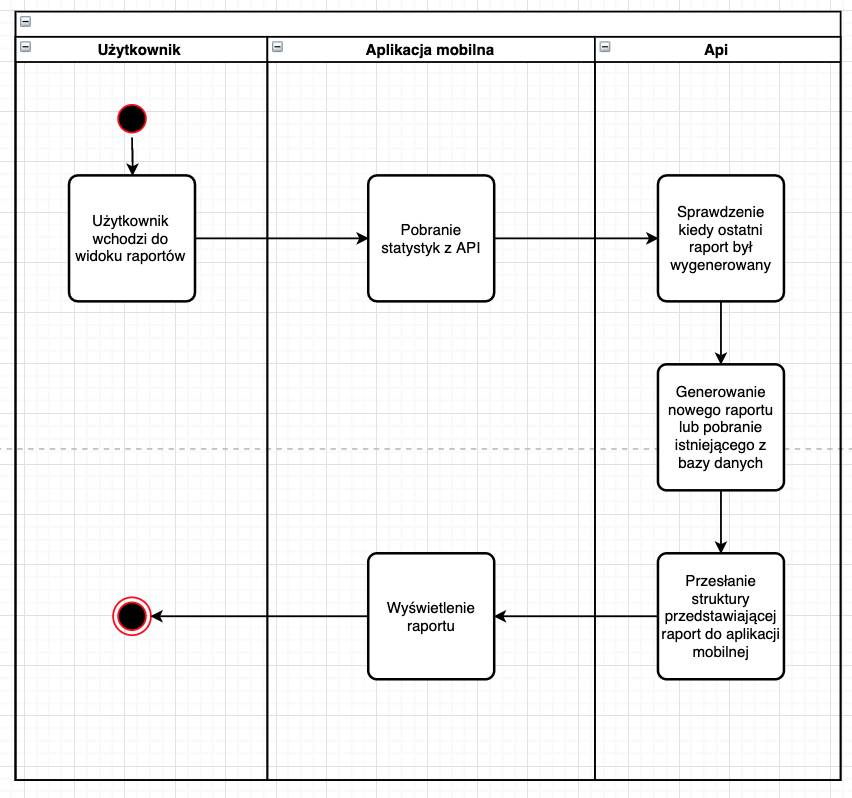
\includegraphics[scale=0.5]{images/raport-uml.png}
    \caption{Diagram przedstawiający proces odczytywania raportu w aplikacji mobilnej.}
    \label{fig:raport_uml}
\end{figure}

\begin{figure}[!htbp]
    \centering
    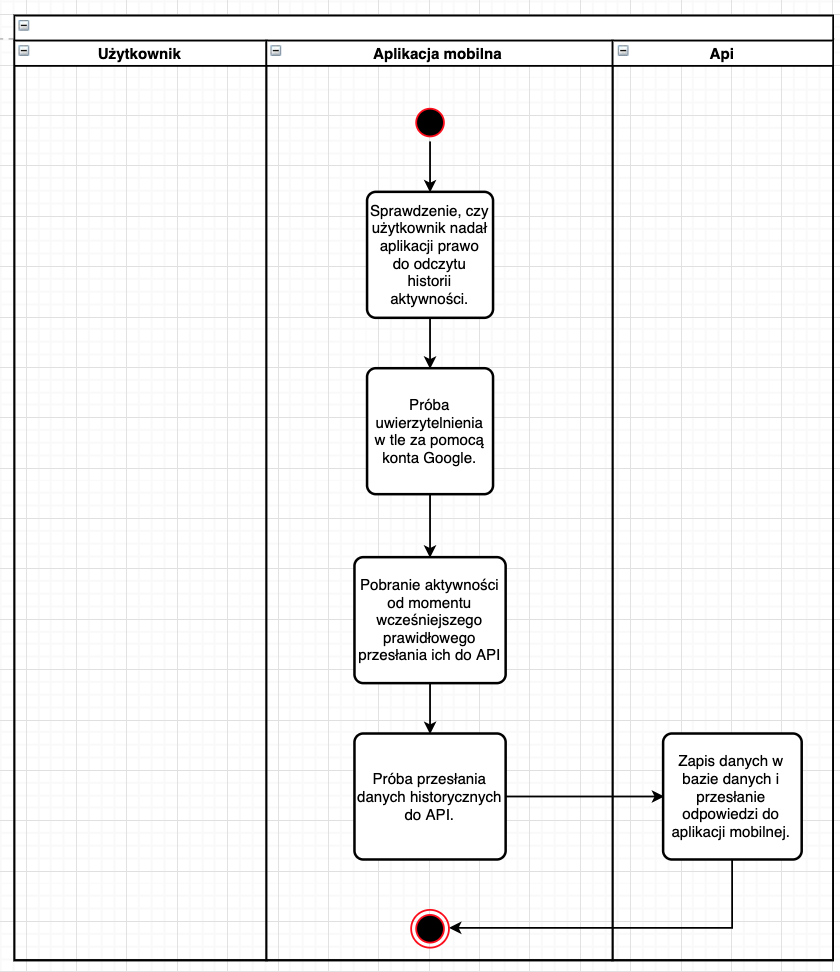
\includegraphics[scale=0.5]{images/cyclic-stats-uml.png}
    \caption{Diagram przedstawiający cykliczny proces przesyłania danych historyczny do serwisu zewnętrznego.}
    \label{fig:cyclic_stats_uml}
\end{figure}

\FloatBarrier

\section{Wymagania niefunkcjonalne}
Sekcja ta przedstawia te elementy z których składa się projekt, a nie są widoczne z perspektywy użytkownika. 
\begin{itemize}
  \item Język programowania dla aplikacji mobilnej: Kotlin.
  \item Użycie biblioteki do uwierzytelnienia poprzez konto google: play-services-auth.
  \item Użycie mechanizmów Alarmu w celu cyklicznych zachowań w aplikacji mobilnej.
  \item Dystrybucja aplikacji w Google play~\cite{publish_app}.
  \item Użycie natywnych mechanizmów systemu Android w celu pozyskania historii aktywności.
  \item Stworzenie serwisu zarządzającego bazą aktywności.
  \item Wybór oraz użycie algorytmu uczenia maszynowego w celu interpretacji historii aktywności.
\end{itemize}

\section{Narzędzia}
Kod źródłowy projektu zarządzany był z użyciem rozproszonego systemu kontroli wersji Git, korzystając z hostingowego serwisu internetowego GitHub. Podczas implementacji aplikacji mobilnej używane było zintegrowane środowisko Android Studio. W celu testowania i debugowania jakości informacji w bazie danych zostało użyte narzędzie DataGrip przeznaczone do pracy z różnego rodzaju bazami SQL. Podczas tworzenia serwisu połączonego z aplikacją mobilną używano edytora programistycznego Visual Studio Code. Natomiast w trakcie implementacji serwisu generującego raport oraz podczas analizy danych i różnych klasyfikatorów użyto zintegrowane środowisko Pycharm przeznaczone dla języka Python. Obserwacja i zarządzanie komunikacją miedzy poszczególnymi jednostkami odbywała się za pomocą serwisów wewnątrz AWS (z ang. \ang{Amazon Web Services}).


\chapter{Specyfikacja zewnętrzna}
\label{chap:zewn}
Rozdział ten przedstawia podstawowe wymagania niezbędne do uruchomienia aplikacji mobilnej stworzonej podczas pracy inżynierskiej. Znajduje się tu również informacja o wszystkich krokach niezbędnych do instalacji i uruchomienia tej aplikacji. Użytkownik może też zapoznać się z tym w jaki sposób korzystać z systemu wybierając jeden z scenariuszy. 
\section{Wymagania sprzętowe, programowe i instalacja}

Aby zainstalować aplikację wymagane jest posiadanie urządzenia mobilnego z systemem Android w wersji przynajmniej 6.0 (Android Marshmallow). Ze względu na komunikacje z serwisami zewnętrznymi, urządzenie musi również posiadać stały dostęp do internetu. W celu pozyskania programu na urządzenie mobilne wystarczy włączyć Play Store i wyszukać aplikację wpisując TrackApps, a następnie wybrać z listy element, którego szczegóły widoczne są na rysunku
\ref{fig:google_play_screen}.

\begin{figure}[h!]
    \centering
    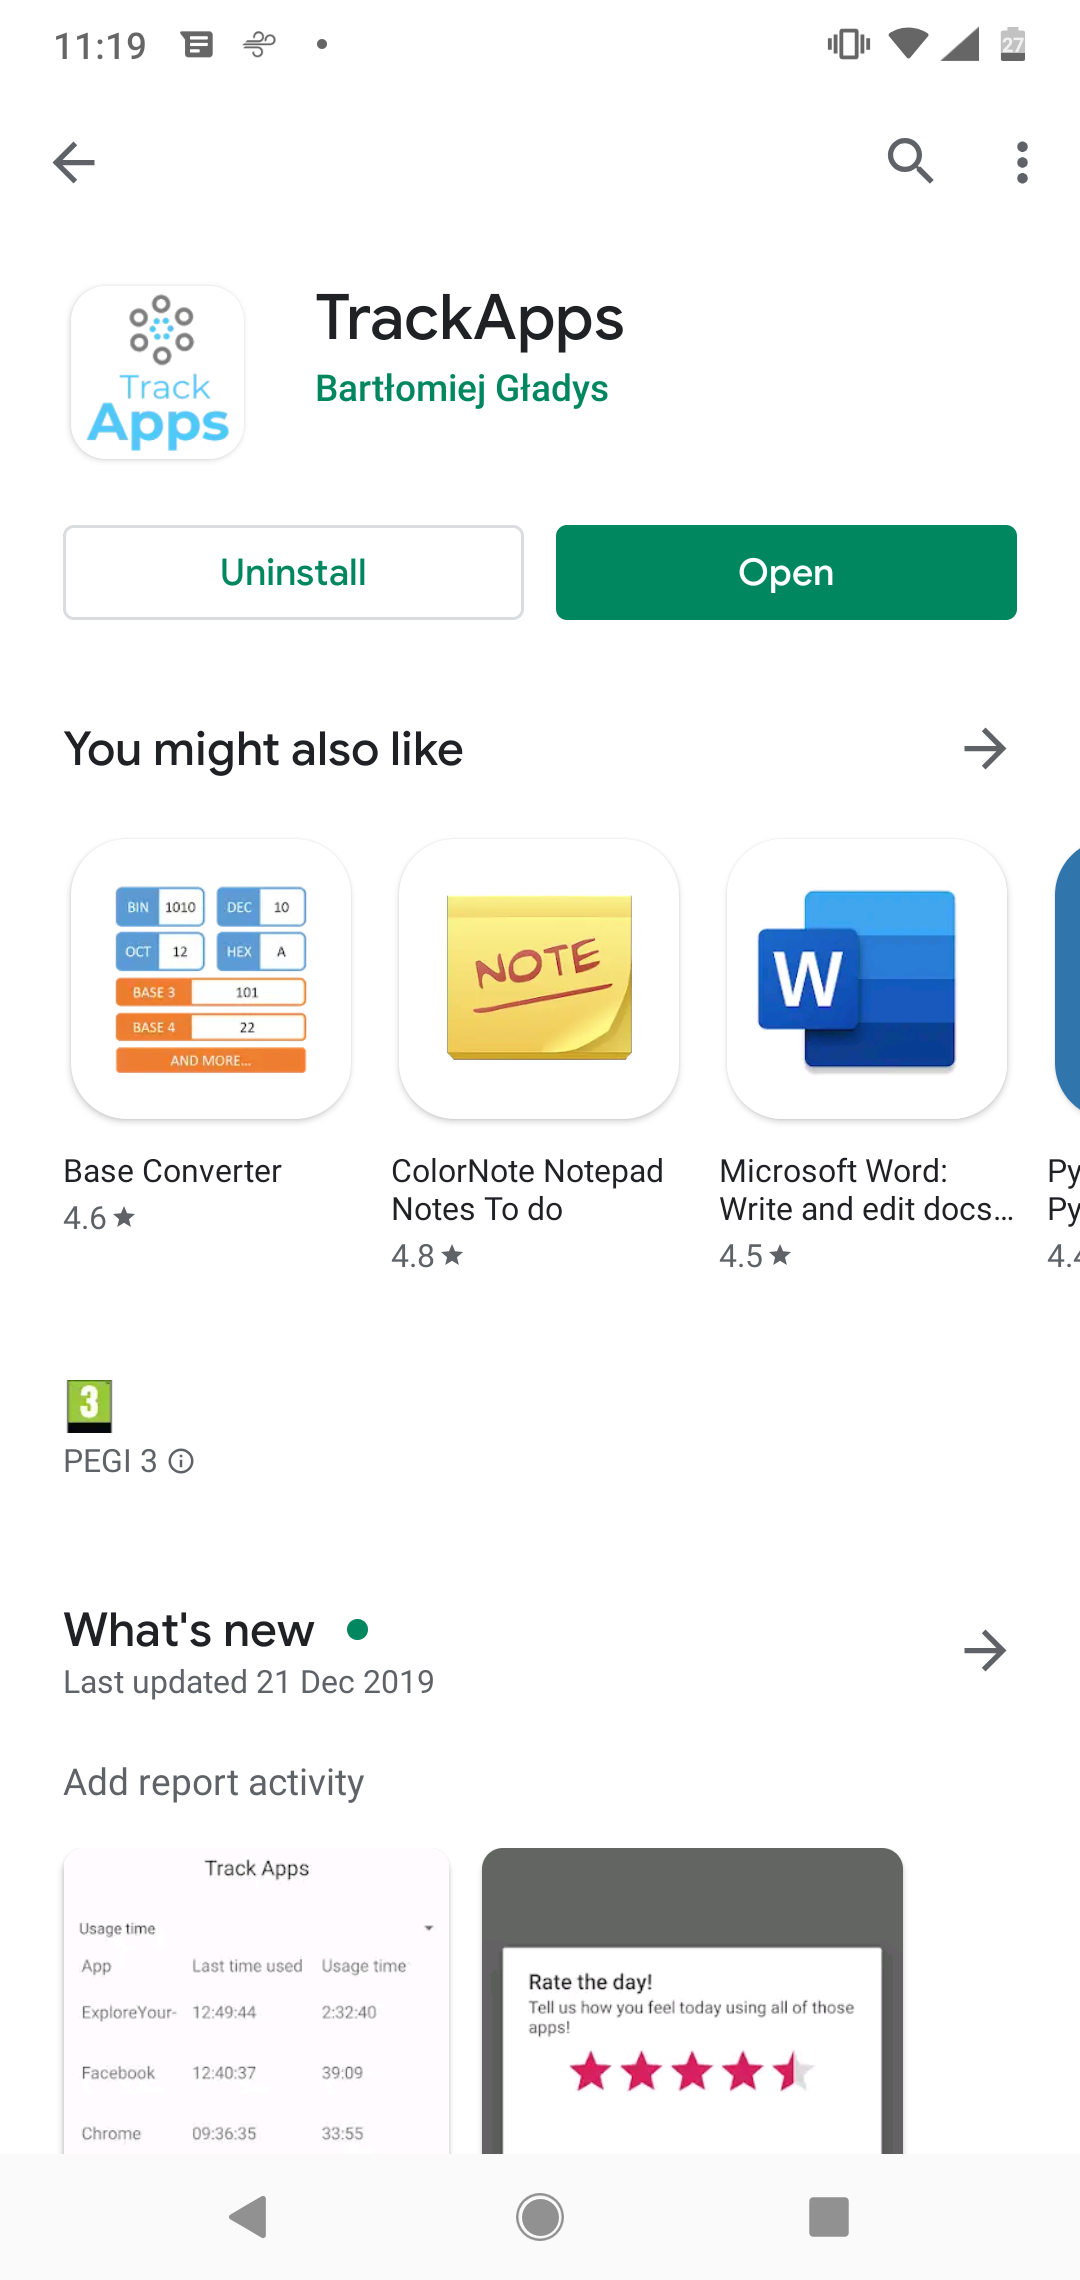
\includegraphics[scale=0.2]{images/google_play_screen.png}
    \caption{Szczegóły aplikacji wykonanej w ramach pracy inżynierskiej w Google Play.}
    \label{fig:google_play_screen}
\end{figure}

Po pomyślnej instalacji użytkownik jest przekierowany do widoku zezwoleń, w którym świadomie musi ustawić aplikacji mobilnej prawo pobierania historii aktywności. Widok procesu znajduje się na przedstawionym rysunku \ref{fig:usage_access}.

\begin{figure}[h!]
    \centering
    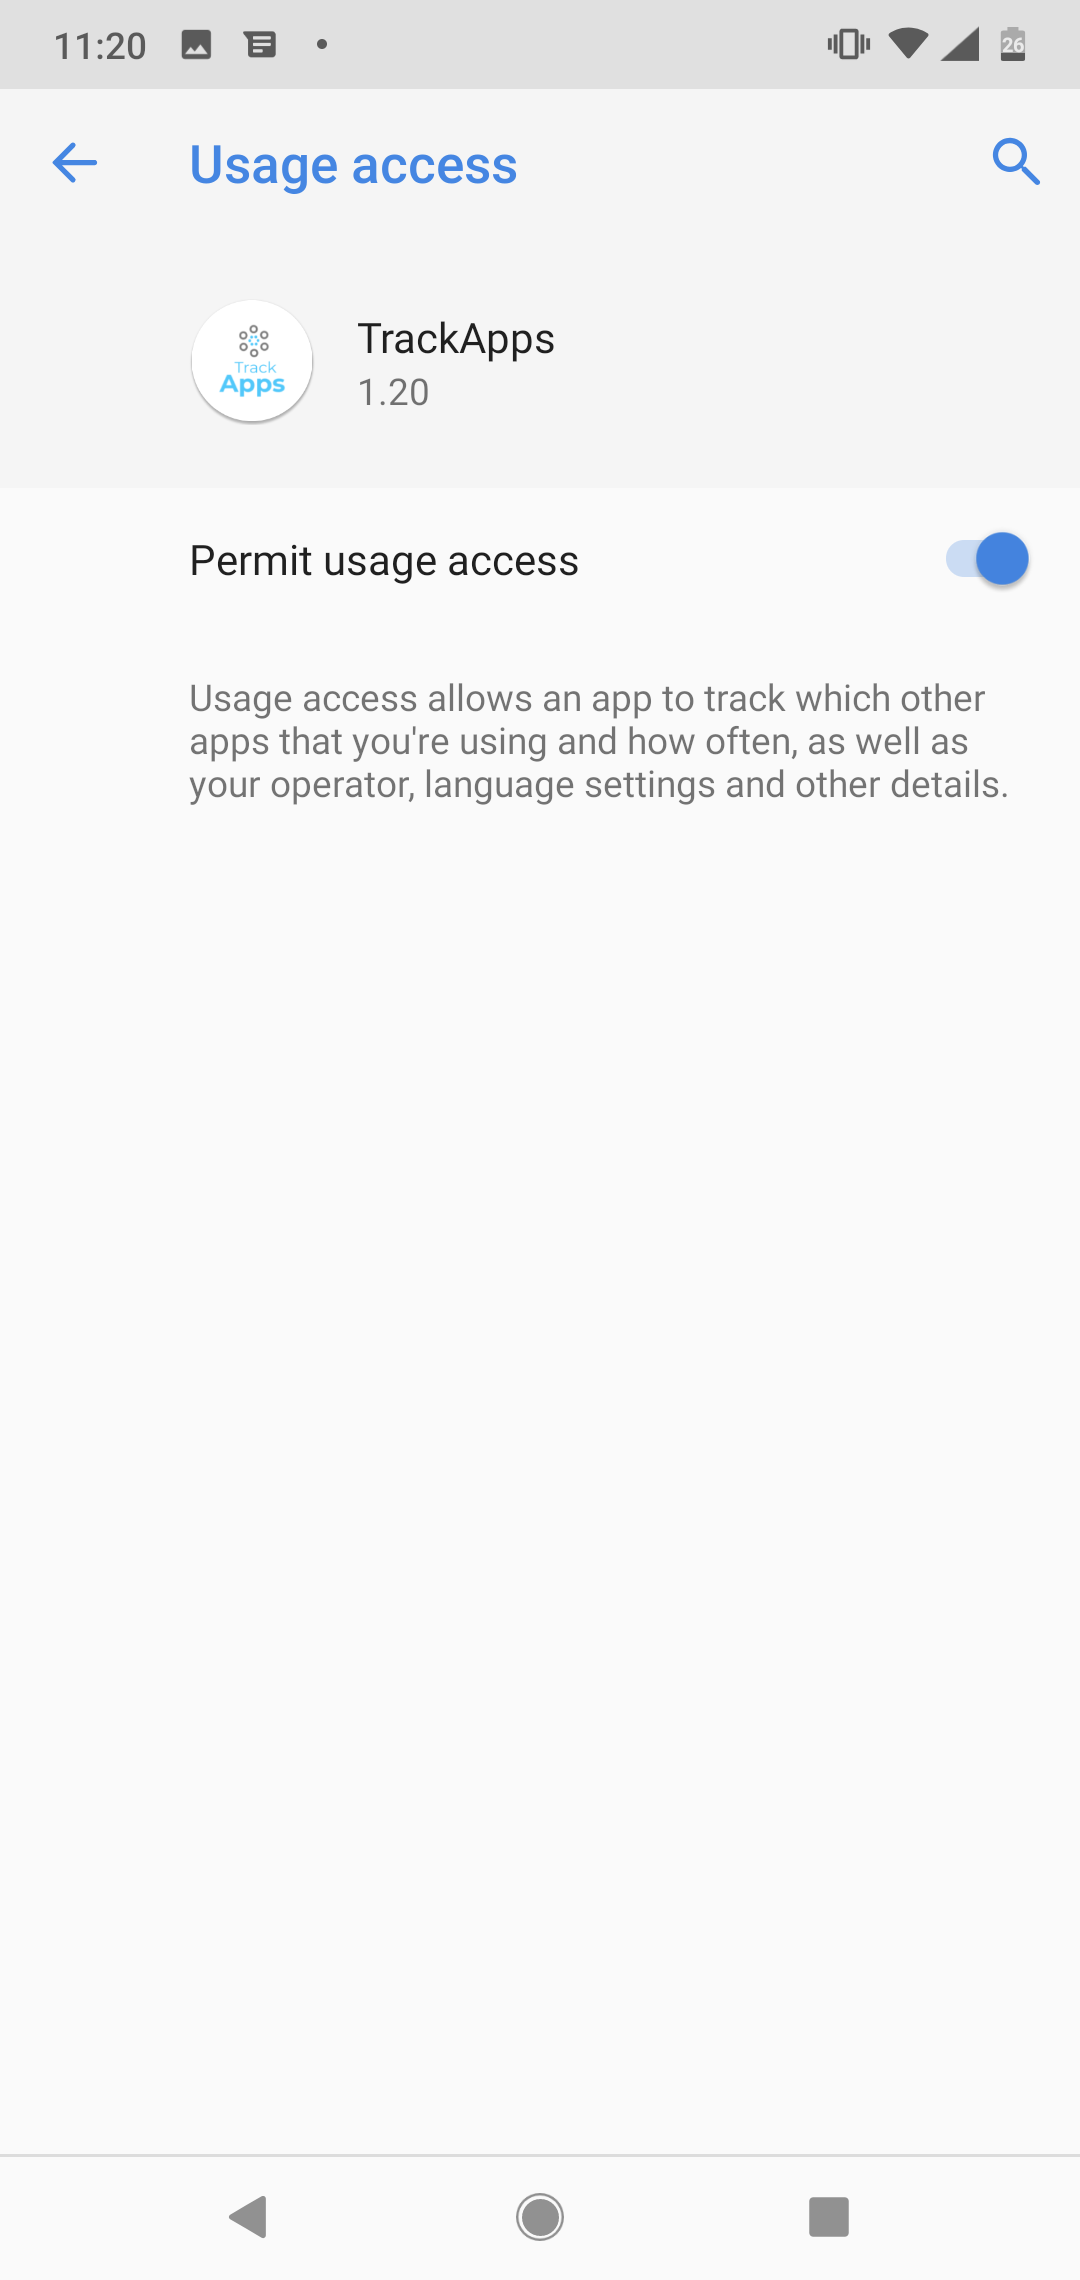
\includegraphics[scale=0.2]{images/usage_access_screen.png}
    \caption{Ustawianie zezwoleń do śledzenia historii aktywności dla aplikacji wykonanej w ramach pracy inżynierskiej.}
    \label{fig:usage_access}
\end{figure}


Następnie wyświetlona zostaje informacja o wymaganej autoryzacji poprzez wybranie konta Google prezentująca się tak jak na rysunku \ref{fig:auth_screen}. Jeżeli użytkownik pozytywnie przejdzie przez wymienione wyżej dwa etapy, na ekranie pojawi się lista z ostatnio odwiedzonymi aplikacjami oraz ilością czasu jaki spędził na danych aktywnościach. Dzięki autoryzacji przez konto Google, użytkownik nie musi wpisywać hasła ani uzupełniać ręcznie swoich danych do logowania, co powoduje, że żadne poufne informacje nie są w stanie wycieknąć przez tę aplikację. Kolejną cechą autoryzacji w ten sposób jest to, że nawet w przypadku gdy użytkownik zmieni urządzenie mobilne to jego wszystkie wpisy historyczne i oceny będą zapisane wewnątrz systemu.

\begin{figure}[h!]
    \centering
    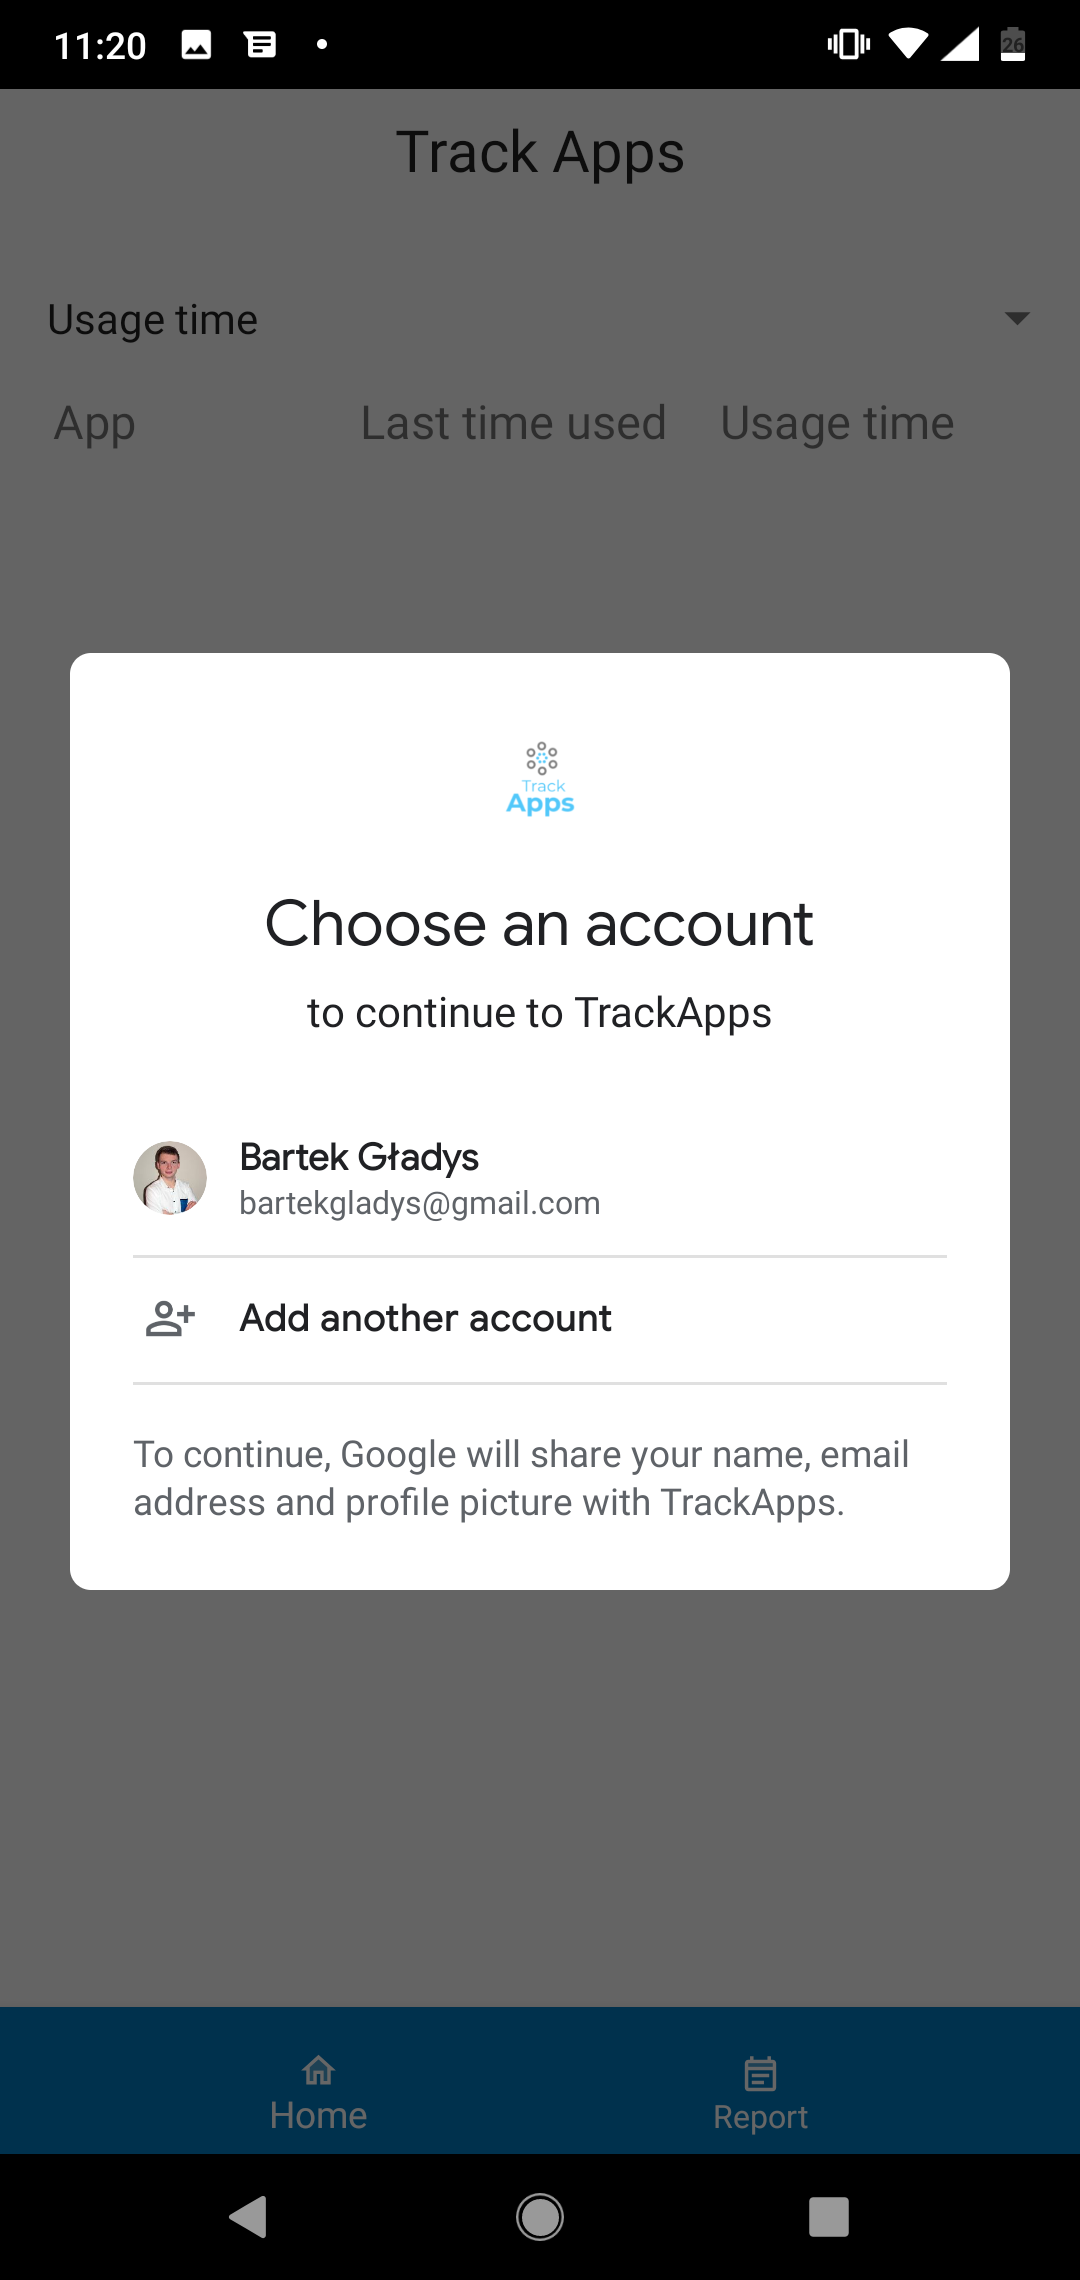
\includegraphics[scale=0.2]{images/account_screen.png}
    \caption{Autoryzacja poprzez korzystanie z usługi Google Play Services wewnątrz aplikacji wykonanej w ramach pracy inżynierskiej.}
    \label{fig:auth_screen}
\end{figure}

\section{Scenariusze korzystania z systemu}
Jedyną aktywnością wymaganą do poprawnego zbierania i klasyfikacji danych jest wpisywanie przez użytkownika oceny samopoczucia w zakresie od 0 do 5. Proces ten jest widoczny na przedstawionym rysunku \ref{fig:rate_screen}. 
\begin{figure}[h!]
    \centering
    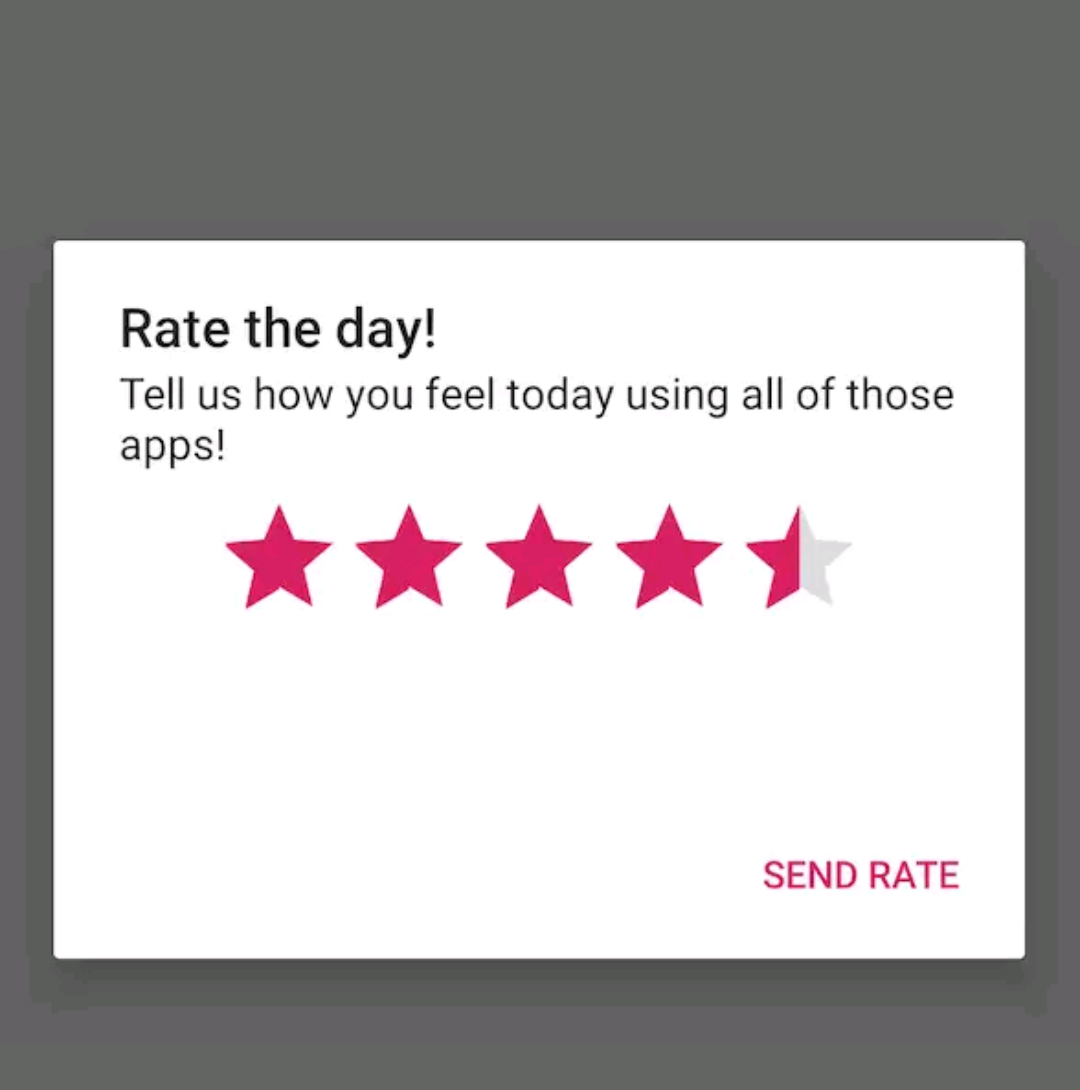
\includegraphics[scale=0.2]{images/rate_screen.png}
    \caption{Widok oceny dnia w aplikacji wykonanej w ramach pracy inżynierskiej.}
    \label{fig:rate_screen}
\end{figure}

Widok ten jest wyświetlony cyklicznie -- raz każdego dnia i nie można go ,,wywołać'' ręcznie poprzez nawigację w programie. Aplikacja posiada dwa standardowe widoki po jakich użytkownik może się poruszać. Pierwszym z nich jest widoczna na zrzucie ekranu \ref{fig:activites_history} lista, która może być sortowana po trzech atrybutach: nazwie programu, spędzonym na aplikacji czasie oraz bazując na tym, która aplikacja była używana ostatnio. 
\begin{figure}[h!]
    \centering
    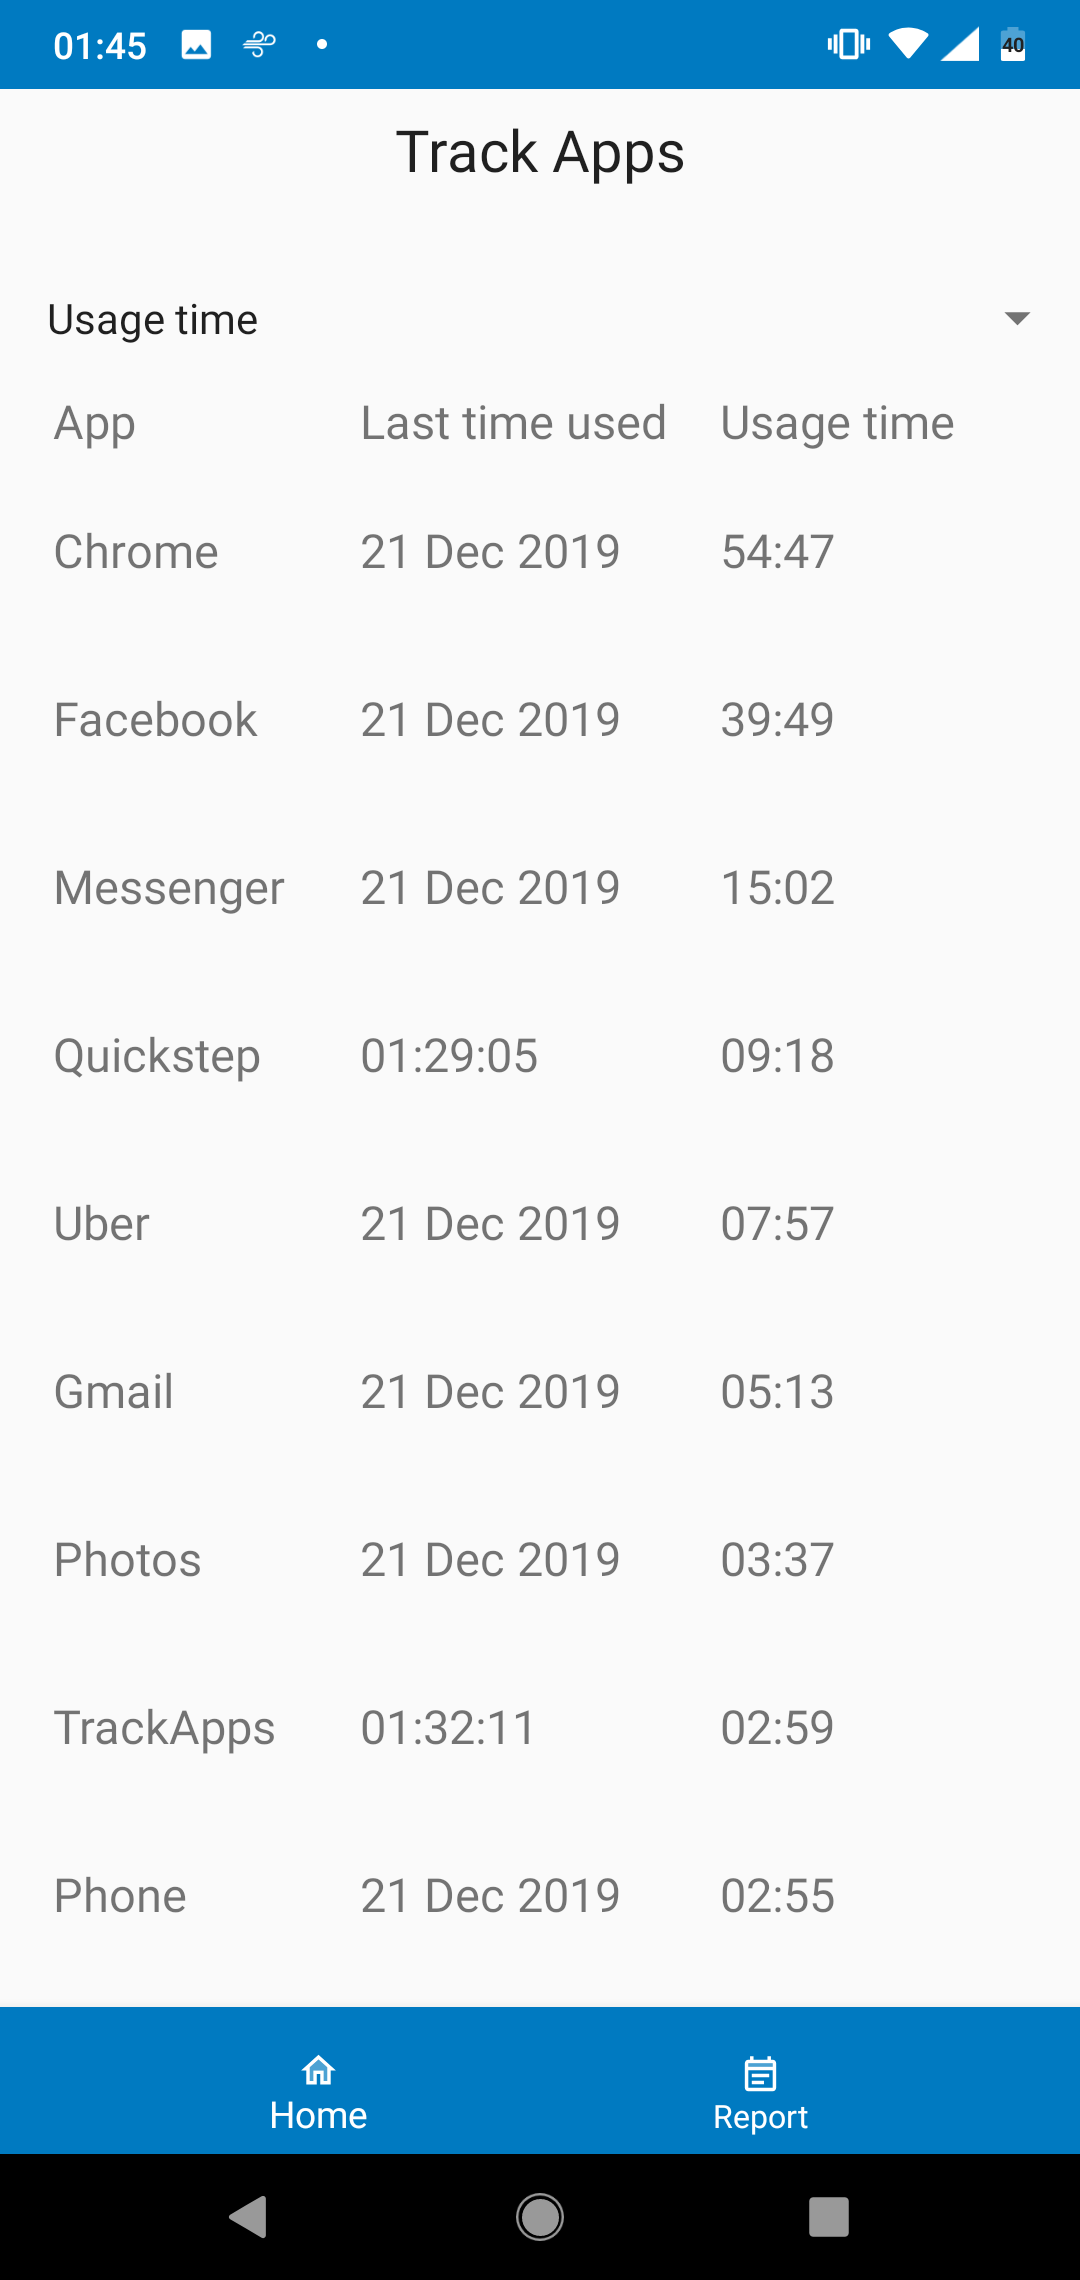
\includegraphics[scale=0.2]{images/activites_history.png}
    \caption{Widok aktywności odbywających się w ostatnich dwudziestu czterech godzinach w aplikacji wykonanej w ramach pracy inżynierskiej. Znajdująca się tu lista pokazuje nazwę aplikacji, ostatni punkt w czasie kiedy użytkownik z niej korzystał, oraz sumę czasu, jaki użytkownik poświęcił danej aplikacji.}
    \label{fig:activites_history}
\end{figure}
Kolejną aktywnością jest widok raportu \ref{fig:report} przedstawiający trzy aplikacje, które uzyskały największe wagi podczas procesu klasyfikacji oraz trzy, które uzyskały najmniejsze. 
\begin{figure}[h!]
    \centering
    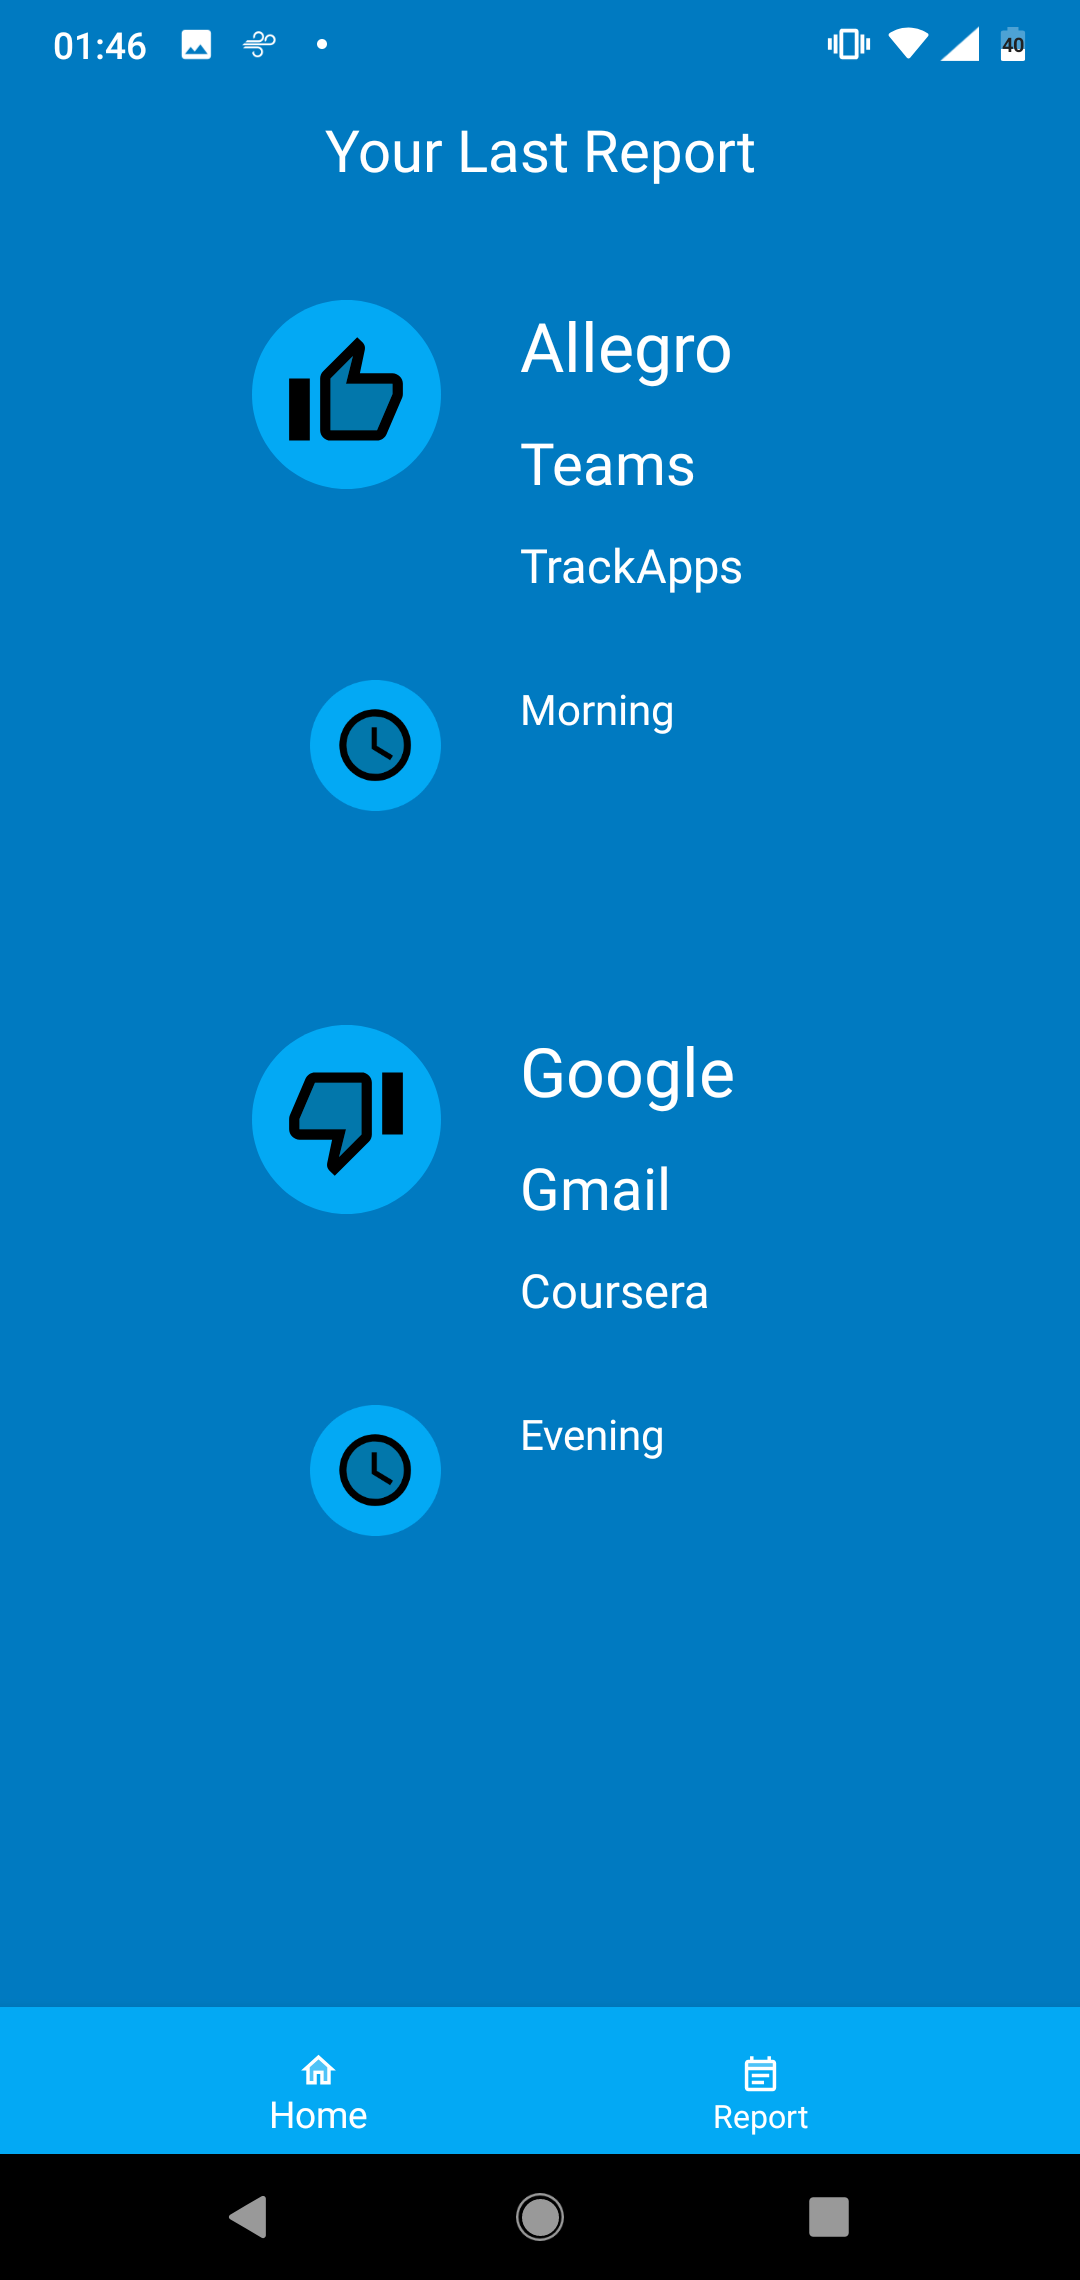
\includegraphics[scale=0.2]{images/report.png}
    \caption{Widok raportu w aplikacji wykonanej w ramach pracy inżynierskiej. Na początku przedstawione są aplikacje, które wpływają pozytywnie na samopoczucie użytkownika oraz pora dnia w której posługiwanie się urządzeniem mobilnym wpływa korzystnie. Analogicznie, poniżej przedstawione są aplikacje które wpływają negatywnie na samopoczucie i pora dnia w ciągu której posługiwanie się urządzeniem mobilnym wpływa niekorzystnie.}
    \label{fig:report}
\end{figure}
Dodatkowo, widnieje tam informacja o tym, jaka pora dnia jest najodpowiedniejsza do korzystania z urządzenia mobilnego oraz przeciwnie o jakich godzinach używanie telefonu wpływa na użytkownika negatywnie. 



\chapter{Specyfikacja wewnętrzna}
\label{chap:wewn}
W tym rozdziale zostaną przedstawione wszystkie elementy które nie są widoczne dla użytkownika, a spełniają fundamentalną rolę w kontekście poprawnego działania całego systemu zbudowanego w ramach pracy inżynierskiej. W pierwszym etapie opisana będzie transformacja historycznych danych aktywności z postaci natywnej dla systemu Android do postaci umożliwiającej klasyfikację. Następnie, w sekcji \ref{models} opisane zostaną algorytmy które były brane pod uwagę podczas wyboru modelu do klasyfikacji. W sekcji \ref{structure} znajdą się informację na temat struktury projektu i tego jak dane serwisy i aplikacja mobilna są ze sobą połączone. W sekcji \ref{mobile} zostaną opisane szczegóły implementacji aplikacji mobilnej. W sekcji \ref{db} będzie przedstawiona struktura bazy danych. Następnie, w sekcji \ref{nodejs} pojawią się informacje na temat serwisu odbierającego dane z urządzeń mobilnych. Finalnie, w sekcji \ref{python} zostaną przedstawione szczegóły dotyczące serwisu zajmującego się analizą danych i tworzeniem raportów.   

\section{Przygotowanie danych}
\label{preparing}
Aby umożliwić klasyfikacje danych na bazie aktywności użytkownika i ocen, które podaje, wymagane było zastosowanie pewnego grupowania wyglądającego następująco. Na samym początku została wykorzystana dyskretyzacja w celu zamiany godziny danej aktywności na porę dnia, np. aktywność, która odbywała się o godzinie 19:00 została przyporządkowana do nominalnej klasy ,,Wieczór'', a aktywność z godziny 12:00 do klasy ,,Południe''. Dzięki takiej zamianie można było w pewien sposób przyspieszyć algorytm oraz uzyskać wyniki lepsze w kontekście interpretacji. Następną kwestią było zagadnienie dotyczące klasyfikacji wszystkich aktywności z jednego dnia do jednego rekordu posiadającego ocenę w tymże dniu. Z tego względu oryginalne dane widoczne w tabeli \ref{tab:orig_activity} zostały przekształcone do wektora danych, który opisuje sumę czasu w sekundach dla każdej aplikacji oraz każdej pory dnia i jest widoczny w tabeli \ref{tab:changed_activity}. Dodatkowo widać, że w procesie transformacji danych użyto kodowanie ,,1 z n''~\cite{one_hot_encoding} zarówno dla nominalnych danych odnośnie pory dnia jak i nazw aplikacji. W ten właśnie sposób było możliwe przygotowanie danych historycznych w jednym wierszu i przypisane ich do oceny którą dany użytkownik udzielił. Następnie użyto regresji logistycznej w celu uzyskania wag dla każdego z atrybutów bazując na ocenie. Klasyfikator oceniał dany przykład jako pozytywny jeżeli prognozowana ocena była równa lub większa średniej wszystkich ocen dotychczasowo wystawionych przez użytkownika. Przykładowo, użytkownik wystawił oceny $1, 2, 3, 4, 5$, średnia tych ocen wynosi $3$, więc w momencie gdy użytkownik przy kolejnej próbie wystawienia oceny wybierze $4$, to model przypiszę do zbioru aktywności z tego dnia klasę pozytywną. Gdyby jednak użytkownik wybrał ocenę $2$, to model przypisał by do danego zbioru klasę negatywną. Podczas początkowej fazy projektu próbowano ten sam problem rozwiązać z użyciem regresji, a więc każdy unikalny zbiór aktywności posiadał by przypisaną ocenę. Niestety, błąd treningowy był na tyle duży, że postanowiono zrezygnować z regresji i jako model wybrano klasyfikator dokonujący wyboru między dwoma etykietami. Więcej informacji na temat działania klasyfikatora regresji logistycznej i innych algorytmów, które były wzięte pod uwagę, znajduję się w następnej sekcji. 

\begin{table}[]
\centering
\caption{Przykładowe dane historyczne pochodzące z Usage Stats API w systemie Android}
\begin{tabular}{|l|l|l|}
\hline
time\_in\_sec                         & name                       & day\_part \\
\hline
10459.658      & youtube & night     \\
8932.143       & youtube & afternoon \\
8860.36        & com.facebook.orca          & night \\
\hline
\end{tabular}
\label{tab:orig_activity}
\end{table}

\begin{table}[]
\centering
\caption{Przykładowe dane historyczne po transformacji z postaci oryginalnej dla Usage Stats API w systemie Android do postaci umożliwiającej klasyfikację}
\begin{tabular}{|l|l|l|l|l|}
\hline
time\_in\_sec & youtube & facebook & day\_part\_night & day\_part\_afternoon \\
\hline
28252.161     & 19391.801                        & 8860.36                 & 19320.018        & 8932.143    \\ 
\hline
\end{tabular}
\label{tab:changed_activity}
\end{table}


\section{Opis algorytmów klasyfikujących}
\label{models}
W tej sekcji zostaną opisane wszystkie z czterech algorytmów, które zostały przetestowane pod kątem jakości uzyskanego modelu. Tymi algorytmami są: regresja logistyczna, $k$-NN (z ang. \ang{k nearest neighbours} -- $k$ najbliższych sąsiadów), drzewo decyzyjne oraz MLP (z ang. \ang{Multilayer Perceptron} -- najpopularniejszy typ sztucznej sieci neuronowej). Więcej informacji na temat samego procesu testowania i walidacji znajduje się w rozdziale \ref{chap:valid}. 

Pierwszy z nich, regresja logistyczna bazuje na funkcji sigmoid wizualnie prezentującej się jako krzywa przypominająca literę ``S`` zdefiniowaną wzorem: 
$
\frac{1}{1 + e^{-y}}
$, gdzie $ y $ to wynik funkcji typu 
$
b_{0} + b_{1}\cdot x_{1} + b_{2}\cdot x_{2} + ... + b_{n}\cdot x_{n}
$, natomiast $ b $ opisuje wagi dla poszczególnych wartości $ x $, gdzie $x_{i}$ to czas wyrażony w sekundach dla pewnej aplikacji $i$. Dla danych opisywanych w tym projekcie $ n $ jest zdefiniowane jako suma wszystkich aplikacji, z których pewny użytkownik korzysta plus liczba etykiet, które opisują porę dnia zależną od godziny używania aplikacji. We wzorze znajduje się jeden wolny element $ b_{0} $ (z ang. \ang{bias}), który definiuje pewną wartość początkową i w przypadku regresji liniowej dla zerowych wartości \textbf{x}, rezultatem będzie właśnie ta składowa.

Kolejny algorytm -- $k$-NN~\cite{knn} jest nieparametryczną metodą klasyfikacji. Bazuje ona na przydzielaniu pewnego elementu do klasy, do której należy większość z jego sąsiadów. Do prawidłowego działania algorytmu trzeba zdefiniować pewną liczbę $k$, która przedstawia liczbę sąsiadów wymaganą by przydzielić dany obiekt do danej klasy. Przedstawiony tutaj model opierał się o hiperparametr $k=3$. Dlaczego więc algorytm $k$-NN jest nazwany metodą nieparametryczną, jeżeli trzeba zdefiniować parametr $ k $? Otóż, podczas uczenia maszynowego występuje rozróżnienie na parametry i hiperparametry. Te pierwsze są dynamiczne i zmieniają się za każdym razem, gdy model jest trenowany i testowany na nowych danych (np. wagi przyporządkowane we wcześniej opisanym modelu regresji logistycznej). Hiperparametry natomiast są ustawiane na początku algorytmu i nie zmieniają się dynamicznie podczas całego procesu. Z uwagi na fakt, że $k$-NN jest metodą nieparametryczną wynika więc, że model ten nie uczy się podczas etapu prognozy, a jest jedynie korygowany za każdym razem gdy dostarczone są nowe dane. 

Drzewo decyzyjne tak samo jak $k$-NN jest modelem nieparametrycznym. Klasyfikator jest tworzony w taki sposób, że atrybuty mające największe znaczenie są bliżej korzenia względem tych, których znacznie jest znikome podczas prognozy klasy wynikowej. Każdy element posiadający rozgałęzienie przedstawia predykat bazujący na atrybucie, a liście drzewa przedstawiają wynik prognozy. Ze względu na to, że atrybuty nie przedstawiają nominalnych danych (na początku była wykonana dyskretyzacja, ale następnie wartości zostały przemnożone przez czas, którego jednostką były sekundy), to jako metoda do wyboru atrybutów na poszczególnych rozgałęzieniach wybrany został współczynnik Giniego~\cite{gini} (z ang. \ang{Gini index}) przedstawiony wzorem:
$
1-\sum_{k=1}^{K}\left ( \frac{\left | C_{k} \right |}{\left | D \right |} \right )^{2}
$, gdzie $ D $ to liczba wszystkich przykładów, a $ C_{k} $ to liczba tych przykładów, które należą do klasy $ k $. Ze wzoru można zauważyć, że czym współczynnik Giniego jest mniejszy, tym rozgałęzienie jest lepsze. Prawdopodobnie powodem tego, że AUC było tak niskie jest mała ilość danych treningowych.

MLP~\cite{mlp}, czyli Sieć neuronowa na ogół składa się z jednej warstwy do wprowadzania danych (z ang. \ang{input layer}), jednej warstwy do wyprowadzania danych (z ang. \ang{output layer}) oraz jednej lub więcej warstw ukrytych (z ang. \ang{hidden layer}). W warstwie ukrytej znajdują się tzw. neurony, które otrzymują dane z warstw poprzednich pomnożone przez pewne wagi ustalane podczas procesu tworzenia sieci, czyli modelu. Neurony po otrzymaniu danych używają z góry zdefiniowanych funkcji aktywacyjnych. Przekształcają one informacje wejściowe i przesyłają je dalej. Cały proces składa się z wielu iteracji, gdzie za jedną iterację uważa się przejście danych przez wszystkie warstwy ukryte aż do warstwy wyjściowej (z ang. \ang{forward propagation}) i etap ,,uczenia''  korygujący wagi pomiędzy warstwami, podczas którego zmiany propagują się od strony wyjściowej do wejściowej (z ang. \ang{back propagation}). Dla sieci użytej w projekcie zostały użyte pewne empirycznie wybrane hiperparametry. Maksymalna liczba iteracji została ustawiona na 1000. Jako funkcje aktywacyjną wybrano $max(0, x)$, często opisaną jako relu (z ang. \ang{rectified linear unit}).
Rozmiar sieci neuronowej to jedna warstwa, w której zawiera się 25 neuronów.

Na początku projektu, planowano również zastosować naiwny klasyfikator bayesowski~\cite{naive}, ale jako że algorytm ten w podstawowej wersji wspiera tylko dane o postaci ,,Prawda/Fałsz'', to odstąpiono od tej decyzji. Wybór algorytmów poddanych eksperymentowi opierał się o popularność w kontekście algorytmów klasyfikacyjnych. Ze względu na to, że wszystkie dane były tworzone i zbierane podczas pracy inżynierskiej, to nie było ich na tyle dużo, aby czas trwania danych algorytmów klasyfikacyjnych był brany pod uwagę podczas wybierania konkretnego modelu. 

\section{Struktura projektu}
\label{structure}
Projekt od strony implementacji został podzielony na trzy części. Jest to aplikacja mobilna napisana w języku Kotlin dla systemów Android, system napisany w środowisku Node.js połączony z bazą danych PostgreSQL w oparciu o infrastrukturę zbudowaną wewnątrz serwisów dostawcy chmurowego AWS, oraz aplikacja analizująca dane i generująca raporty napisana w języku Python. Na diagramie \ref{fig:general} przedstawiono komunikację pomiędzy poszczególnymi elementami systemu. Natomiast, w tabeli \ref{tab:libs} znajdują się wszystkie biblioteki wykorzystane bezpośrednio podczas implementacji.  

Wszystkie komponenty poza aplikacją mobilną znajdują się wewnątrz AWS. Aplikacje bezpośrednio komunikujące się z bazą danych są uruchomione wewnątrz klastra EC2 (z ang. \ang{Amazon Elastic Compute Cloud})~\cite{ec2}, czyli serwisie www, który dostarcza skalowalną moc obliczeniową w chmurze. Interfejs wystawiony przez aplikacje napisaną w środowisku Node.js jest głównym źródłem komunikacji dla aplikacji mobilnej. Natomiast serwis napisany w języku Python posiada interfejs, z którego korzysta jedynie wcześniej opisany serwis na potrzeby tworzenia i zapisywania w bazie danych raportów. 

Dodatkowo, warto zwrócić uwagę na serwis CodeDeploy \& CodePipeline, który ułatwia pracę programiście poprzez wprowadzanie automatycznej budowy aplikacji. W momencie kiedy pojawia się nowa zmiana na serwerze git, natychmiastowo zostaje o tym poinformowany owy serwis i wykonuje wszystkie niezbędne skrypty po stronie klastra EC2, które umożliwiają ściąganie zależności, zainstalowanie pakietów i zbudowanie aplikacji. Inną zaletą skorzystania z serwisów AWS i klastra EC2, jest łatwość obsługi i połączenia systemu z bazą danych, oraz możliwość zarządzania otwartymi i zamkniętymi portami, dzięki czemu aplikacja pozostaje bezpieczna udostępniając w sieci tylko niezbędne zasoby.      

\begin{figure}[h!]
    \centering
    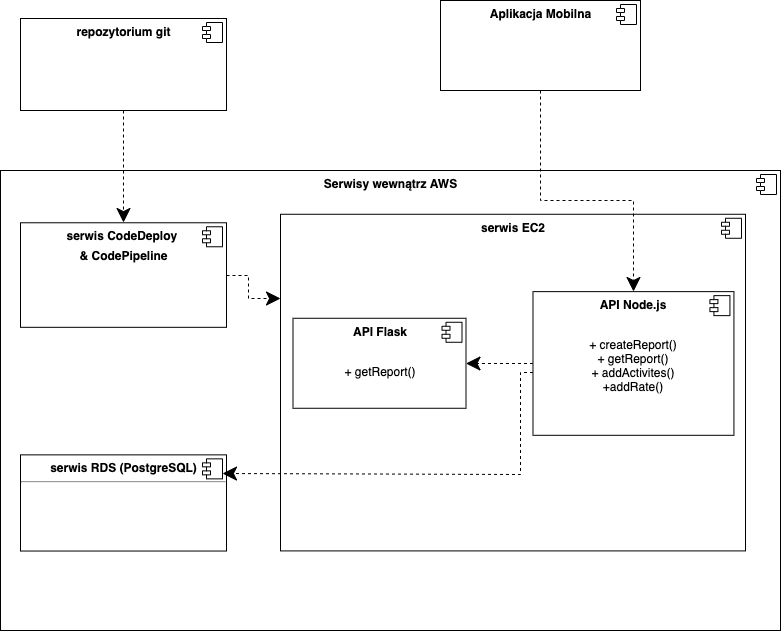
\includegraphics[width=\textwidth]{images/general_diagram_track_apps.png}
    \caption{Infrastruktura projektu.}
    \label{fig:general}
\end{figure}



\section{Aplikacja mobilna}
\label{mobile}
Aplikacja została napisana w języku Kotlin przy użyciu środowiska Android Studio i wydana na platformie Google Play, aby ułatwić zbieranie danych i instalowanie aplikacji przez potencjalnych użytkowników.
Na diagramie \ref{fig:mobile_uml} widać, że aplikacja posiada trzy aktywności (widoki na jakie użytkownik może się natknąć). 

Pierwszym z nich jest \textit{MainActivity}, gdzie użytkownik ma dostęp do listy z historią wszystkich aplikacji jakich używał podczas ostatnich dwudziestu czterech godzin. Na potrzeby wyświetlania listy została stworzona klasa \textit{UsageStatsAdapter}, która rozszerza natywną klasę \textit{BaseAdapter} dodając nowe funkcje, takie jak: sortowanie po nazwie aplikacji, sortowanie po ostatniej dacie uruchomienia i sortowanie po czasie spędzonym na danej aplikacji. W celu implementacji sortowania w aplikacji stworzono trzy klasy pomocnicze istniejące wewnątrz klasy \textit{UsageStatsComparator} rozszerzające funkcjonalność generycznej klasy \textit{Comparator}. Klasa ta również implementuje metodę \textit{getView}, która pobiera wszystkie niezbędne informacje z listy aktywności i przekazuje je do widoku listy, która zostanie wygenerowana. Dodatkowo, następuje tutaj pozyskanie nazwy aplikacji bazując na nazwie modułu, który został zapisany w bazie danych dla konkretnego programu, oraz formatowanie daty z postaci zapisanej w milisekundach do postaci łatwej do przeczytania i rozpoznania. 

Pobraniem historii wszystkich aplikacji zajmuje się klasa \textit{UsageStatsUtil}, która konwertuje dane w taki sposób aby były łatwiejsze do wyświetlenia, czy też przesłania do innych serwisów. Implementacja logiki zajmującej się konwersją danych znajduje się w metodzie \textit{fetchStatsDataForExternal}. Metoda ta pobiera listę zdarzeń, które odbyły się na urządzeniu mobilnym w przekazanym przez parametr okresie czasu, wykorzystując przy tym natywną klasę \textit{UsageStats}. Następnie odbywa się filtrowanie przekazujące dalej jedynie te zdarzenia, które miały wpływ na użytkownika i są one opisane flagami \textit{MoveToForeground} -- flaga mówiąca o tym, że aplikacja pojawiła się na głównym planie urządzenia mobilnego, \textit{MoveToBackground} -- flaga mówiąca o tym, że dana aplikacja została zminimalizowana. Gdy zdarzenia są już pobrane i przefiltrowane, następuje sortowanie i konwersja do typu listy, gdzie każdy element składa się z dwóch zdarzeń o różnych flagach, które zostały opisane wcześniej. Dodatkowymi funkcjami tej aktywności jest sprawdzenie czy użytkownik nadał aplikacji mobilnej prawo do pobrania historii statystyk oraz weryfikacja stanu uwierzytelnienia z serwisem Google Auth~\cite{auth_api}. Jeżeli użytkownik uruchamia aplikację po raz pierwszy to pojawi się modalne okno dialogowe z wyborem konta Google przez które chciałby się zalogować do aplikacji, następnie zostanie on przekierowany do widoku ustawień urządzenia mobilnego, gdzie będzie musiał zaznaczyć odpowiednie ustawienia dla tej aplikacji. Mechanizm uwierzytelnienia został napisany w klasie \textit{ApiHandler} i bazuje na bibliotece play-services-auth. Natomiast mechanizm, który powoduje przejście do widoku ustawień został stworzony za pośrednictwem natywnej klasy \textit{UsageStatsManager}~\cite{usage_stats_api} i mechanizmu intencji, dzięki czemu istnieje możliwość przekierowania użytkownika z aplikacji do widoku ustawień. 

Za kolejny widok w aplikacji mobilnej odpowiada klasa \textit{ReportActivity}. Tak samo jak we wcześniejszym przypadku, używane są zależności z klasy \textit{ApiHandler}. Natomiast w tym momencie poza metodą \textit{authenticate}, używana jest również metoda \textit{getReport}, która pozwala na pobranie przypisanego do konta ostatniego raportu w bazie danych i możliwość wyświetlenia go w aktywności. W raporcie widnieje informacja o tym jakie aplikacje działały na użytkownika pozytywnie, a jakie negatywnie. Znajduje się tu również informacja o tym jaka pora dnia powinna być bardziej sprzyjająca w kontekście użytkowania urządzenia mobilnego. Metoda \textit{getReport} jak i metody, które opisane zostaną w dalszej części (\textit{rate}, \textit{sendStats}) zostały zaimplementowane przy użyciu biblioteki Fuel, która znacznie ułatwia wykonywanie żądań do serwisów zewnętrznych za pomocą protokołu HTTP. Warto dodać, że biblioteka pozwala również na łatwe skorzystanie z wzorca projektowego jakim jest Interceptor w celu dodania dodatkowych funkcjonalności do każdego żądania. Wykorzystując ten wzorzec można w łatwy sposób ,,udekorować`` pewną metodę w dodatkową funkcjonalność, która zostanie wykonana przed lub po wywołaniu. W przypadku tej aplikacji mobilnej Interceptor ma za zadanie wstrzykiwać odpowiedni nagłówek HTTP za każdym razem gdy następuje komunikacja z serwisem zewnętrznym, dzięki czemu zostaje przesłana informacja na temat aktualnie zalogowanego użytkownika. 

Za ostatni widok w aplikacji jest odpowiedzialna klasa \textit{AlertActivity}, ta aktywność nie jest dostępna z widoku menu w aplikacji, natomiast cyklicznie każdego dnia pojawia się na urządzeniu mobilnym użytkownika z zapytaniem o ocenę samopoczucia. Do komunikacji z serwisem zewnętrznym w celu przesłania wybranej przez użytkownika oceny służy po raz kolejny klasa \textit{ApiHandler} oraz metoda \textit{rate}. Codzienne wywoływanie komunikatu w postaci aktywności zostało zaimplementowane w klasie \textit{AlarmReceiver}, która rozszerza natywny \textit{BroadcastReceiver}~\cite{alarm_api} wprowadzając funkcjonalność nasłuchiwania na wywołanie intencji z systemu Android. Wyzwalacz akcji bazuje na natywnym mechanizmie alarmów,  pozwala on  o wybranej godzinie uruchomić wybraną funkcję. Implementacja tego rozwiązania opiera się o nadpisanie bazowej metody \textit{onReceive} dodając funkcjonalność, która nasłuchuje na dany typ intencji. Jeśli takowa intencja się pojawi, zostanie stworzona nowa, do której przypisana będzie flaga informująca o tym, że powinno zostać stworzone nowe zadanie i finalnie nowo stworzona intencja zostanie przesłana jako argument do metody \textit{startActivity} w kontekście uzyskanym z parametru \textit{onReceive}. 

Poza widokami w aplikacji mobilnej warto też wyszczególnić mechanizm, który cyklicznie wysyła dane na temat historii użytkowania do serwisu zewnętrznego. Mechanizm ten korzysta także z funkcji natywnego alarmu oraz w znacznej mierze z wcześniej opisanych metod \textit{authenticate} i \textit{sendStats} z klasy \textit{ApiHandler}. Metody te są wykorzystywane w celu autoryzacji z serwisem zewnętrznym gdy aplikacja działa w tle oraz w celu przesłania historycznych aktywności. Implementacja tego rozwiązania również opiera się o dodanie warunku nasłuchującego na konkretną intencję. Gdy takowa się pojawi, w pierwszym kroku zostanie utworzona nowa instancja typu \textit{UsageStatsManager}. Następnie, obiekt ten zostanie przesłany jako źródło informacji razem z pewnym domyślnym odcinkiem czasu do wcześniej wspomnianej metody \textit{fetchStatsDataForExternal}. Przed samym wysłaniem żądania uzyskane dane zostaną przekształcone do formatu JSON używając przy tym biblioteki Gson, aby w ostatnim kroku użyta została statyczna metoda \textit{sendStats} na obiekcie \textit{API}, która wyśle żądanie HTTP POST pod adresem \textit{activites} serwisu zewnętrznego.
\begin{figure}[h!]
    \centering
    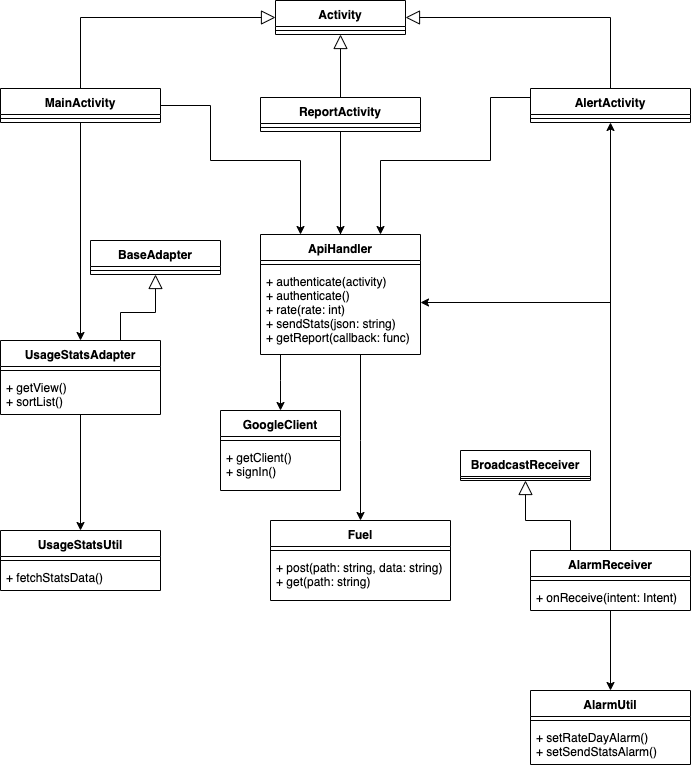
\includegraphics[width=\textwidth]{images/track-app-mobile-diagram.png}
    \caption{Diagram przedstawiający zależności między klasami w aplikacji mobilnej.}
    \label{fig:mobile_uml}
\end{figure}
\section{Baza Danych}
\label{db}
Silnikiem bazodanowym, który został wybrany jest już wcześniej napomniany PostgreSQL. Głównym atutem tego narzędzia jest ogromna liczba dostępnych typów danych i funkcji pomagających w pewien sposób te dane konwertować. Na diagramie \ref{fig:bd} widać podział bazy danych na cztery tabele.

Pierwsza z nich, application, opisuje zbiór wszystkich aplikacji rozpoznawanych w systemie. Dzięki takiej reprezentacji danych bezproblemowo można sprawdzać, jak często dana aplikacja była uruchamiana przez użytkownika oraz z technicznego punktu widzenia zachować wysoki poziom normalizacji bazy danych. 

Kolejna z nich, user, przechowuje informacje na temat adresu email, wieku, punktu w czasie kiedy to dany użytkownik został stworzony w bazie danych oraz raportu przechowywanego jako typ JSON~\cite{psqjson} (JavaScript Object Notation), czyli obiektu który posiada swoje własne atrybuty i jest dowolnie zagnieżdżony. Można by pomyśleć, że wybór takiego typu danych ogranicza funkcjonalność i elastyczność tabeli, natomiast w tym przypadku tworzeniem struktury całego atrybutu raport zajmuje się inny system, a baza danych pełni jedynie role, w której przyporządkuje ostatni raport do użytkownika, dzięki czemu może być on wyświetlony w aplikacji mobilnej. Niestety, relacja posiadająca atrybut w tej formie nie spełnia pierwszej postaci normalnej. Z uwagi na fakt, że atrybut report jest jednostką zagnieżdżoną, encja user posiada nieelementarne wartości. 

Tabela rating posiada numeryczne pole rating przyjmujące wartości między 0, a 5. Posiada również pole date w celu zapisania daty kiedy dana ocena została zapisana. Znajduje się tu również klucz obcy tabeli user, dzięki któremu można przypisać ocenę do danego użytkownika.

Pomiędzy tabelami user i application, na podstawie tabeli activity, jest stworzona relacja ,,wiele do wielu``. Poza kluczami obcymi wymaganych relacji, występują tu również pola from i to, które bezpośrednio informują o tym, w jakich godzinach dana aktywność występowała.



\begin{figure}[h!]
    \centering
    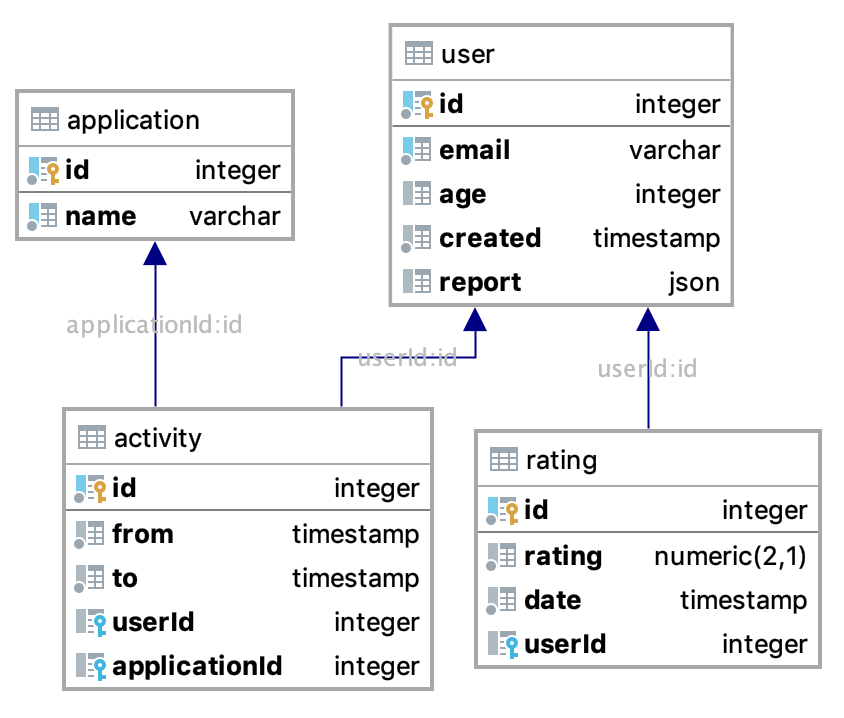
\includegraphics[width=\textwidth]{images/db_schema.png}
    \caption{Diagram przedstawiający schemat bazy danych.}
    \label{fig:bd}
\end{figure}


\section{Serwis zarządzający bazą danych i obsługą żądań z aplikacji mobilnych}
\label{nodejs}
Aplikacja została napisana przy pomocy środowiska Node.js oraz języka TypeScript, który jest kompilowany prosto do postaci zgodnej z standardem JavaScript. Wybór ten został podjęty ze względu na możliwość używania silnego typowania, które nie jest dostępne w natywnej wersji JavaScript. Dodatkowo TypeScript wspiera wiele rozszerzeń nie uwzględnionych w  specyfikacji JavaScript np. interfejsy, czy też wyliczeniowe typy danych, które pomagają opisać implementacje zgodnie domeną problemu. Jedyną wadą wspomagania się silnym typowaniem w środowisku Node jest przymus do kompilowania kodu po każdej zmianie, ale istnieją narzędzia, które ułatwiają ten proces i pozwalają na dynamiczne wyprodukowanie wersji wynikowej w bardzo krótkim czasie.

Dodatkowo, podczas implementacji projektu zostały użyte biblioteki pomocnicze. Jedną z nich jest typeorm~\cite{typeorm} i jak nazwa wskazuje zapewnia ona mapowanie obiektowo-relacyjne, co powoduje, że obsługa bazy danych po stronie serwisu jest w większym stopniu odseparowana od silnika bazodanowego. Przewagą typeorm nad innymi rozszerzeniami tego typu jest bardzo dobre wsparcie dla języka TypeScript, dzięki czemu statyczna analiza kodu źródłowego może być w pełni wykorzystana. Inną, niemniej ważną zaletą tej biblioteki jest wsparcie dla wielu paradygmatów programowania, które można użyć w różnych przypadkach i przy inny poziomie trudności projektu. Jednym z nich jest wzorzec obiektowy aktywnego rekordu, dzięki któremu podstawowe metody do zarządzania danymi mogą być automatycznie wygenerowane. Niestety wzorzec ten jest ściśle zintegrowany z strukturą bazy danych i praktycznie zaciera granice między warstwą przechowującą dane, a logiką domenową, dlatego też podczas implementacji użyto wzorca Repozytorium. Jest on bardzo dobrze wspierany przez typeorm i umożliwia seperację między wymienionymi powyżej warstwami, poprzez tworzenie tzw. repozytorium, osobno dla każdego obiektu domenowego w projekcie.

Inną kluczową biblioteką jest google-auth-library, która konwertuje i weryfikuje nagłówki przychodzących żądań z aplikacji mobilnych dzięki czemu możliwe jest przypisanie użytkownika do danych historycznych. Na samym końcu, przy samej obsłudze wymiany informacji z klientami mobilnymi oraz innymi serwisami w całym procesie pomocne są biblioteki takie jak axios oraz express. Pierwsza z nich umożliwia wysyłanie żądań HTTP do innych aplikacji, natomiast druga sprawia, że w łatwy sposób można utworzyć REST API (interfejs pozwalający zarządzać zasobami serwisu) oraz wstrzykiwać zależności, które będą wykonywać pewne transformacje na danym żądaniu i przekazywać je dalej. 

Na diagramie \ref{fig:backend_uml} widać podział ze względu na serwisy, które zajmują się pewną częścią logiczną systemu i spotykają się dopiero w miejscu gdzie aplikacja tworzy interfejs, z którego mogą skorzystać inni klienci. Zaczynając od lewej strony, pierwszy widnieje serwis \textit{Activity}, który umożliwia dodanie danych historycznych przez aplikacje mobilną. Korzysta on z dwóch repozytoriów \textit{Activity} oraz \textit{Application}, ponieważ dane są te bezpośrednio połączone. Serwis zapisuje ile razy i jak długo użytkownik korzystał z danej aplikacji więc istnieje tu relacja jeden do wielu, gdzie dla jednego obiektu typu \textit{Application} przydzielonych jest wiele obiektów typu \textit{Activity}. Wyżej opisane repozytoria korzystają z klas typu \textit{Entity}, które odzwierciedlają postać tabel w bazie danych. Widać tu jednak bardzo istotną różnicę w reprezentacji relacji, ponieważ obiekt typu \textit{Application} posiada referencję do listy aktywności co nie miałoby miejsca w modelu czysto relacyjnym. 

Kolejna gałąź diagramu przedstawia serwis Rating, który jest odpowiedzialny za obsługę ocen  przychodzących z urządzeń mobilnych. Tak samo jak we wcześniejszym przypadku jest podział na serwis, repozytorium oraz strukturę odpowiadającą tabeli Rating z bazy danych. 

Ostatnią częścią aplikacji jest funkcjonalność odpowiadająca za tworzenie spersonalizowanych raportów. W tym miejscu główny serwis przed stworzeniem raportu w bazie danych używa wcześniej wymienionej biblioteki axios w celu utworzenia żądania HTTP i wysłania go do systemu zajmującego się przetworzeniem danych. Jako rezultat operacji zwrócony zostanie model, będący w stanie przedstawić aplikacje wpływające na użytkownika pozytywnie i negatywnie.

\begin{figure}[h!]
    \centering
    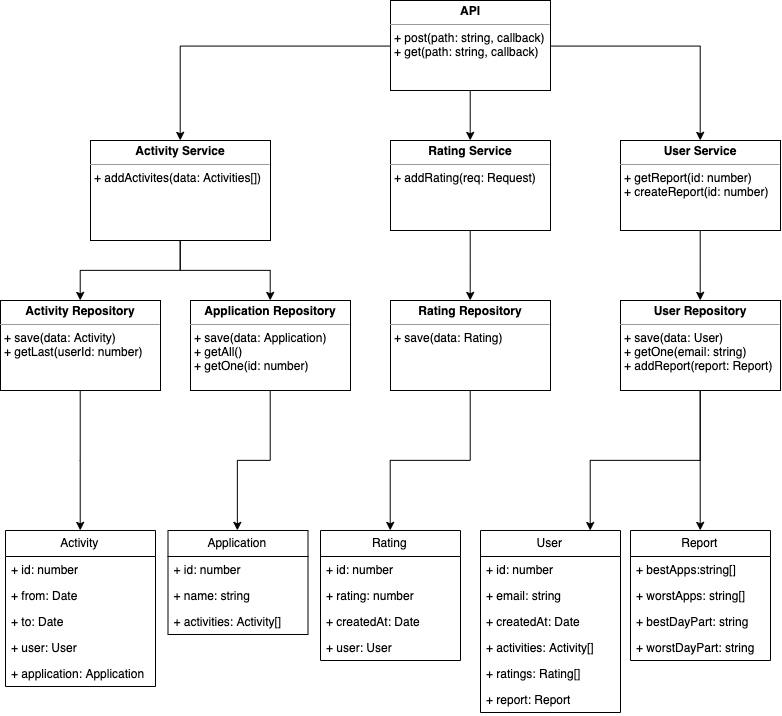
\includegraphics[width=\textwidth]{images/track_apps_backend_diagram.png}
    \caption{Diagram przedstawiający zależności między elementami w aplikacji Node.js.}
    \label{fig:backend_uml}
\end{figure}

\section{Serwis odpowiedzialny za analizę danych i generowanie raportów}
\label{python}
Aplikacja została napisana w języku Python ze względu na dużą liczbę gotowych do użycia narzędzi wspomagających transformacje danych oraz uczenie maszynowe. Wśród wykorzystanych bibliotek znajdują się biblioteki takie jak numpy oraz pandas. Pozwalają one w łatwy sposób operować na danych dostarczając funkcje umożliwiające operacje na macierzach, czy też funkcje działające na wektorach.
Do komunikacji z bazą danych nie zostało użyte rozszerzenie mapujące relacje na obiekty, a zwykły adapter zgodny z silnikiem PostgreSQL o nazwie psycopg2. W celu stworzenia systemu klasyfikacyjnego, który będzie mógł przetworzyć statystki na predykcję i odpowiednio je zinterpretować, wykorzystana została biblioteka sklearn. Aby umożliwić połączonemu z aplikacjami mobilnymi serwisowi łatwy dostęp do tworzenia raportów, użyto również bibliotekę Flask w celu udostępnienia interfejsu będącego w stanie przyjąć żądania HTTP. 

Diagram \ref{fig:ml_uml} przedstawia zależności między częściami tego systemu. Na górze znajduje się obiekt mający na celu jedynie udostępnienie wcześniej opisanego interfejsu pod zadaną ścieżką. Po otrzymaniu identyfikatora użytkownika, przesyła on go dalej do adaptera mającego kontakt z obiektami odpowiedzialnymi za pobranie i wstępne przetworzenie danych oraz zwrócenie niezbędnych danych dla raportu. Obiekt \textit{Preparation} jest bezpośrednio połączony z bazą przez opisany wcześniej adapter psycopg2. Wywołuje on zapytanie SQL zwracające aktywności użytkownika o podanym identyfikatorze, a następnie modyfikuje pobrane dane tworząc dodatkowe atrybuty w celu dyskretyzacji. Dalej tworzone jest kolejne zapytanie SQL w celu pobrania wszystkich ocen jakie dany użytkownik podał wewnątrz aplikacji mobilnej. Na samym końcu wywoływana jest funkcja mająca za zadanie pogrupować dane w odpowiednim formacie, zgodnym z interfejsem biblioteki pandas. 

Po pobraniu i przekształceniu wierszy z bazy danych użyty jest obiekt \textit{LogisticRegressionAdapter} odpowiadający za pobieranie nazw aplikacji wpływających na użytkownika pozytywnie i negatywnie. Implementacja ta opiera się o klasyfikator regresji logistycznej importowany z wcześniej wspomnianej biblioteki sklearn~\cite{logistic_regression}. W trakcie wywołania metody \textit{predict} i \textit{fit}, algorytm przyporządkuje do każdego atrybutu (w tym kontekście atrybut oznacza pewną aplikację, która występuje w historii aktywności użytkownika) specjalne wagi, które są mnożone przez ilość sekund poświęconych na daną aplikację. Wagi te zmieniają się dynamicznie w momencie gdy do systemu dodana jest nowa ocena i określają czy dana aplikacja działa pozytywnie, czy też negatywnie na samopoczucie docelowego użytkownika.

\begin{figure}[!htbp]
    \centering
    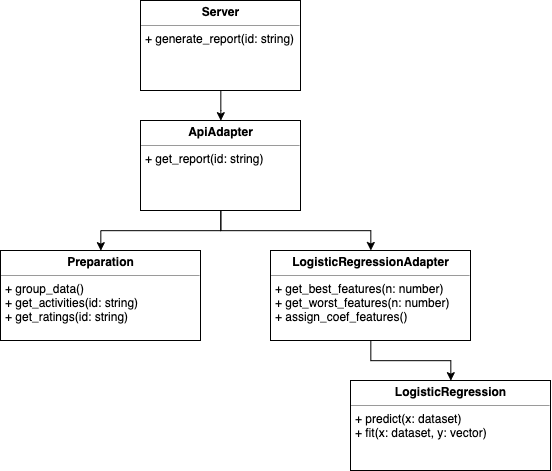
\includegraphics[width=\textwidth]{images/track_apps_ml.png}
    \caption{Diagram przedstawiający zależności między elementami w aplikacji napisanej w języku Python.}
    \label{fig:ml_uml}
\end{figure}


\begin{table}[]
\centering
\caption{Tabela przedstawiająca wszystkie biblioteki które zostały bezpośrednio użyte podczas implementacji.}
\begin{tabular}{|l|l|}
\hline
Nazwa Biblioteki     & Opis Biblioteki                                                                                                                                       \\ \hline
\multicolumn{2}{|l|}{\textbf{Aplikacja Mobilna (Android)}}                                                                                                                   \\ \hline
fuel                 & Biblioteka ułatwiająca tworzenie żądań HTTP.                                                                                                          \\ \hline
google-play-services & \begin{tabular}[c]{@{}l@{}}Biblioteka połączona z serwisem Google Auth \\ umożliwiająca uwierzytelnienie poprzez użycie \\ konta Google.\end{tabular} \\ \hline
gson                 & \begin{tabular}[c]{@{}l@{}}Biblioteka ułatwiająca transformacje danych \\ do postaci JSON i z postaci JSON do natywnych \\ obiektów.\end{tabular}     \\ \hline
\multicolumn{2}{|l|}{\textbf{\begin{tabular}[c]{@{}l@{}}Serwis zarządzający bazą danych i obsługą \\ żądań z aplikacji mobilnych (Node.js)\end{tabular}}}                    \\ \hline
typeorm              & \begin{tabular}[c]{@{}l@{}}Biblioteka umożliwiające stosowanie mapowanie \\ obiektowo-relacyjnego w bazach danych.\end{tabular}                       \\ \hline
express              & \begin{tabular}[c]{@{}l@{}}Biblioteka ułatwiająca obsługę żądań HTTP \\ przychodzących do serwisu.\end{tabular}                                       \\ \hline
axios                & Biblioteka ułatwiająca tworzenie żądań HTTP.                                                                                                          \\ \hline
google-auth          & \begin{tabular}[c]{@{}l@{}}Biblioteka umożliwiająca walidację nagłówków \\ żądań HTTP.\end{tabular}                                                   \\ \hline
\multicolumn{2}{|l|}{\textbf{\begin{tabular}[c]{@{}l@{}}Serwis odpowiedzialny za analizę danych \\ i generowanie raportów (Python)\end{tabular}}}                            \\ \hline
numpy                & \begin{tabular}[c]{@{}l@{}}Biblioteka dostarczająca wiele funkcji pomocniczych, \\ które ułatwiają operacje na wektorach i macierzach.\end{tabular}   \\ \hline
pandas               & \begin{tabular}[c]{@{}l@{}}Biblioteka pozwalająca w łatwy sposób operować \\ na zbiorach danych.\end{tabular}                                         \\ \hline
flask                & \begin{tabular}[c]{@{}l@{}}Biblioteka ułatwiająca obsługę żądań HTTP \\ przychodzących do serwisu.\end{tabular}                                       \\ \hline
sklearn              & \begin{tabular}[c]{@{}l@{}}Biblioteka dostarczająca gotowe do użycia \\ algorytmy z zakresu uczenia maszynowego.\end{tabular}                         \\ \hline
psycopg2             & \begin{tabular}[c]{@{}l@{}}Biblioteka pozwalająca połączyć się z bazą \\ danych o silniku PostgreSQL.\end{tabular}                                    \\ \hline
\end{tabular}
\label{tab:libs}
\end{table}
 





\chapter{Weryfikacja i walidacja}
\label{chap:valid}
Rozdział ten opisuje sposoby weryfikacji i walidacji stworzonego projektu. W pierwszej sekcji opisany został proces testowania i praktyki umożliwiające łatwiejsze budowanie serwisów oraz połączeń między nimi. W kolejnej sekcji przedstawiona została analiza pozwalająca wybrać najbardziej wydajny algorytm klasyfikujący.

\section{Proces testowania serwisów}
Testowanie wszystkich serwisów połączonych z bazą danych w znacznym stopniu było powiązane z serwisami AWS. Przez cały czas trwania projektu silnik bazy danych nie był zainstalowany lokalnie. Wszystkie dane były przechowywane i testowane wewnątrz serwisu RDS (z ang. \ang{Amazon Relational Database Service}), a na urządzeniu lokalnym używano jedynie zintegrowanego środowiska DataGrip, aby uzyskać zdalne połączenie z bazą. W momencie implementacji każdego z serwisów, pozostałe serwisy działały zawsze w obszarze AWS. Dodatkowo jak wspomniano wcześniej podczas opisu struktury systemu, używano podejścia CI/CD~\cite{cicd} (ang. \ang{Continuous Integration / Continuous Delivery}). Pozwala ono na automatyczne budowanie aplikacji. Przyczyniło się to do szybkiej weryfikacji czy oprogramowanie działa poprawnie. Natychmiastowo po każdej zmianie w serwisie, który udostępnia API widoczna była różnica w zachowaniu aplikacji mobilnej. 

\section{Porównanie i wybór algorytmu użytego do klasyfikacji}
Biorąc pod uwagę ilość danych w innych eksperymentach z wykorzystaniem uczenia maszynowego można stwierdzić, że w tym przypadku danych było stosunkowo mało (w ciągu jednego miesiąca dla jednego użytkownika można było uzyskać maksymalnie 30 ocen, czyli 30 wierszy w bazie danych). 

W celu wytrenowania modelu oraz sprawdzenia jaki klasyfikator sprawdza się najlepiej użyto $k$-krotnej walidacji krzyżowej dla $k=5$. Podczas tego procesu zbiór danych jest podzielony na $k$ równych co do wielkości podzbiorów, gdzie każdy z nich raz pełni role podzbioru testowego i $k-1$ razy role podzbioru treningowego. Ze względu na to, że nie należy się spodziewać zbalansowanych danych (czasem może być więcej przykładów pozytywnych, oznaczających wysokie samopoczucie, a czasem więcej negatywnych, oznaczających niskie samopoczucie), nie został użyty taki wskaźnik jak trafność (z ang. \ang{accuracy}). Miary tej nie stosuje się w przypadku zbiorów niezbalansowanych w problemach klasyfikacyjnych, ponieważ klasyfikacja wszystkich przykładów do jednej klasy da i tak wysoką wartość tej miary. Z tego względu jako parametr określający jakość danego klasyfikatora użyto rozmiar pola (AUC -- z ang. \ang{area under the curve}) pod krzywą ROC (z ang. \ang{Receiver Operating Characteristic}), która jest funkcją odcięcia przedstawiającą TPR (z ang. \ang{True Possitive Rate} -- miara pokrycia) w zależności od FPR (z ang. \ang{False Possitive Rate} -- poziom błędu na podstawie przykładów fałszywie przewidzianych jako prawdziwe)~\cite{auc_roc}. Eksperymentom zostały poddane 4 klasyfikatory: regresja logistyczna, $k$-NN (z ang. \ang{k nearest neighbours} -- $k$ najbliższych sąsiadów), drzewo decyzyjne oraz MLP (z ang. \ang{Multilayer Perceptron} -- najpopularniejszy typ sztucznej sieci neuronowej). Szczegółowe informacje o każdym z algorytmów oraz parametry jakie zostały dla nich zastosowane przedstawiono w rozdziale \ref{chap:wewn}.

Wszystkie wykresy dotyczące eksperymentu posiadają tą samą strukturę. Każdy z nich składa się pięciu składowych, które powstały podczas walidacji krzyżowej, jednej wynikowej będącej średnią wszystkich elementów oraz linii diagonalnej pomocnej podczas wizualnego określania jaką jakość posiada dany model. Jeżeli wynik modelu rozstrzygającego problem dwuklasowy znajduje się w pobliżu tej linii, oznacza to, że skuteczność danego klasyfikatora jest bardzo zła i równie dobrze zachował by się klasyfikator działający na podstawie losowania między dwoma klasami. Dodatkowo wykresy przedstawiają informacje na temat AUC oraz odchylenia standardowego. W implementacji części programu zajmującej się generowaniem raportu wybrano regresję logistyczną widoczną na wykresie \ref{fig:plot_logit} ze względu na wysoką wartość średniej AUC względem innych algorytmów oraz łatwość interpretacji modelu.

Przez interpretowalność modelu~\cite{interpr} rozumie się to, w jaki sposób dany algorytm dotarł do pewnych rezultatów. Jako, że regresja logistyczna jest modelowana jako liniowa funkcja, to z łatwością można uzyskać znaczenie danego atrybutu w całym procesie i dowiedzieć się, czy wysoka wartość tego atrybutu wpłynie na pozytywną lub negatywną prognozę (atrybuty posiadające wagi ujemne będą sugerowały negatywną prognozę, a wagi dodatnie odwrotnie). 

\begin{figure}[h!]
    \centering
    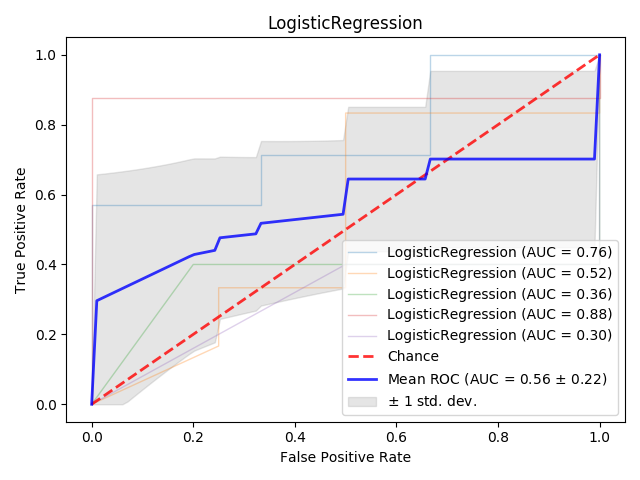
\includegraphics[width=\textwidth]{images/logistic_regression.png}
    \caption{Wykres przedstawiający AUC dla regresji logistycznej.}
    \label{fig:plot_logit}
\end{figure}

Podobny wynik uzyskano używając modelu $k$-NN widocznego na wykresie \ref{fig:plot_knn}, jednak intepretowalność, będąca kluczową jednostką w tym projekcie była zdecydowanie lepsza dla regresji. 
\begin{figure}[h!]
    \centering
    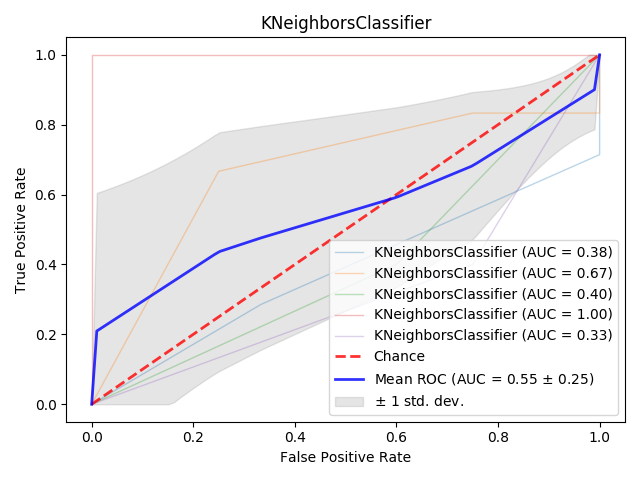
\includegraphics[width=\textwidth]{images/knn.png}
    \caption{Wykres przedstawiający AUC dla KNN.}
    \label{fig:plot_knn}
\end{figure}

Kolejnym algorytmem posiadającym bardzo dobrą interpretowalność jest drzewo decyzyjne którego wyniki pokazane są na rysunku \ref{fig:plot_tree}. AUC tego klasyfikatora rozwiązującego problem dwuklasowy wynosi mniej niż 0.5 co oznacza, że model częściej wskazywał klasę przeciwną.
\begin{figure}[h!]
    \centering
    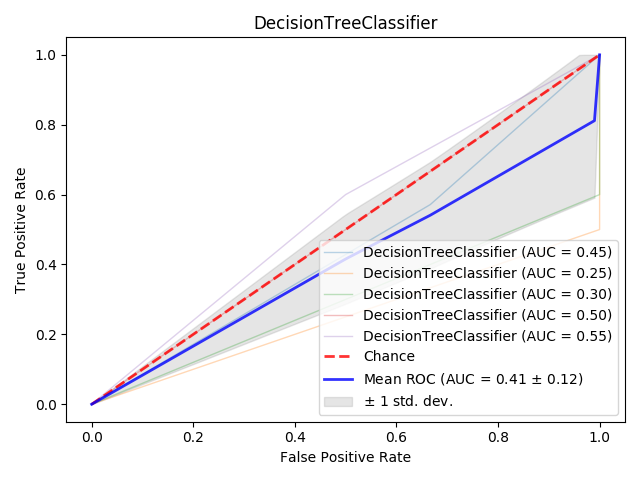
\includegraphics[width=\textwidth]{images/tree.png}
    \caption{Wykres przedstawiający AUC dla drzewa decyzyjnego.}
    \label{fig:plot_tree}
\end{figure}

Ostatnim modelem poddanym eksperymentowi jest MLP, dla którego wyniki są widoczne na rysunku \ref{fig:plot_mlp}. Model ten uzyskał największą średnią AUC, ale jego interpretacja jest dużo trudniejsza niż w przypadku regresji logistycznej.
\begin{figure}[h!]
    \centering
    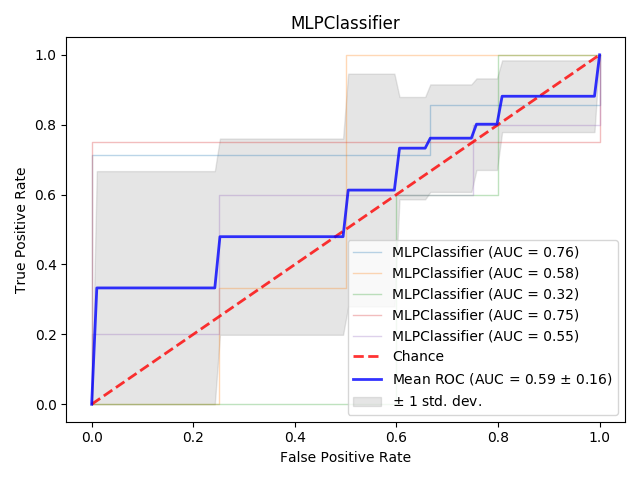
\includegraphics[width=\textwidth]{images/mlp.png}
    \caption{Wykres przedstawiający AUC dla MLP.}
    \label{fig:plot_mlp}
\end{figure}

Eksperymenty można uznać za udane, ponieważ na początku projektu pojawiły się wątpliwości, czy w jakikolwiek sposób można przewidzieć samopoczucie użytkownika biorąc pod uwagę jedynie to z jakich aplikacji on korzystał i w jakiej porze dnia. Maksymalne AUC (dla algorytmu MLP) wynoszące $0.59$ nie jest liczbą wysoką, ale na pewno spisuje się lepiej niż klasyfikacja polegająca na losowaniu między dwoma etykietami.  


\chapter{Wnioski i napotkane problemy}
\label{chap:conc}
Zadanie w ramach pracy inżynierskiej niewątpliwie pozwoliło na zgłębienie wielu technologi i rozwiązań codziennie stosowanych w wielu profesjonalnych projektach. Udało się osiągnąć cel pracy, którym było stworzenie narzędzia umożliwiającego zapisanie i analizę historycznych aktywności użytkownika wewnątrz urządzenia mobilnego. Udało się również zebrać te dane, co wymagało zainstalowania aplikacji na kilku urządzeniach i przekonania innych osób do czynnego oceniania swojego samopoczucia, gdy tylko pojawiała się notyfikacja. Kwestią sporną może być powodzenie klasyfikacji danych, ponieważ AUC będące głównym miernikiem jakości modelu, opisane w rozdziale \ref{chap:valid}, wynosiło jedynie $0.59$. Trzeba jednak pamiętać, że na samopoczucie użytkownika wpływa wiele innych czynników, a same aplikacje mobilne nie są jedynym czynnikiem technologicznym. Użytkownik może również używać aplikacji desktopowych, czy też korzystać większość czasu z przeglądarki internetowej lub oglądać telewizję. Klasyfikator użyty w projekcie nie ma pojęcia o innych aspektach życia użytkownika. Wszystkie dane pochodzą z historii aktywności i ocen wystawianych przez właściciela urządzenia mobilnego, a więc można uznać, że uzyskana wartość jest wynikiem zadowalającym.

Analiza danych mogła zostać w pełni przeprowadzona dzięki kompleksowemu API dostarczonemu przez system Android w urządzeniach mobilnych. Przed i w trakcie implementacji pojawiło się jednak wiele wątpliwości i problemów technicznych, które musiały zostać rozwiązane. 

Jednym z nich było niecodzienne zachowanie natywnego mechanizmu do pobierania historii aktywności. API to nie posiada wbudowanego rozwiązania do powiadomienia o tym, czy dany użytkownik aktualnie zezwolił na pobieranie tych informacji. Mechanizm ten nie zwraca także wyjątku w momencie gdy aplikacja próbuje pobrać dane historyczne nie mając na to pozwolenia, a jedynie pustą listę. Trzeba było więc wykorzystać ten fakt i w momencie gdy zapytanie zwracało pustą listę aktywności zaimplementowano przejście bazujące na mechanizmie intencji do widoku ustawień. W widoku tym użytkownik świadomie musi zaznaczyć prawidłową opcję. 

Kolejnym problemem związanym z wspomnianym API była pewna niekonsekwencja odnośnie zwracania danych historycznych. Specjalny mechanizm przeznaczony do pobierania listy aktywności bazujący na pewnym przedziale czasowym omijał niektóre elementy z listy i dlatego też pojawiła się potrzeba użycia bardziej imperatywnej funkcjonalności tego API. Działa ona w ten sposób, że można pobrać pewne zdarzenia i przefiltrować je po pewnych flagach (flaga przedstawia rodzaj zdarzenia np. ,,użytkownik wszedł do aplikacji'' lub ,,użytkownik wyszedł z aplikacji''). W taki też sposób zostało zaimplementowane pobieranie aktywności. Zdarzenia były pobierane, filtrowane i następnie chronologicznie segregowane aby uzyskać ciągły przebieg wszystkich aktywności odbywających się na urządzeniu mobilnym dla konkretnego użytkownika. 

Innym problemem jaki musiał zostać rozwiązany było nieprawidłowe uwierzytelnianie użytkownika podczas cyklicznych prób pobierania historii aktywności i wysyłania ich do serwisu zewnętrznego, który mógł je potem bezpiecznie zapisać w bazie danych. Rozwiązaniem tego problemu było użycie innej metody dostępnej w bibliotece play-services-auth do autoryzacji, która działa na podstawie zapisanych w pamięci podręcznej ustawień związanych z wcześniej zalogowanym użytkownikiem. 

Kolejnym problemem napotkanym podczas tworzenia aplikacji mobilnej była kwestia niepoprawnie działającej autoryzacji, gdy aplikacja była pobrana z sklepu Play. Podczas instalowania biblioteki zapewniającej uwierzytelnianie dzięki kontu Google wymagane było podanie klucza, który służył do podpisywania programu wynikowego ze względu na bezpieczeństwo. Okazało się, że aplikacja w momencie pojawienia się w sklepie Play jest podpisana jeszcze raz innym kluczem dostępnym z panelu konsoli Play i w tym też momencie moduł odpowiedzialny za autoryzacje przestał działać. Rozwiązaniem tego problemu było stworzenie kolejnego klienta dla biblioteki play-services-auth i warunkowa zmiana identyfikatora zależnie od tego czy aplikacja była budowana i instalowana przez plik .apk, czy też instalowana prosto z sklepu Play. 

Wracając do samej analizy danych, a konkretnie klasyfikacji i jej jakości można było się spodziewać dość niskiego wyniku z tego powodu, że zbierane dane pochodzą jedynie z jednego źródła. Aby takie badania były przeprowadzone dokładniej, dany użytkownik musiałby udostępnić również informacje na temat tego ile czasu przeznacza na korzystanie z aplikacji komputerowych oraz stron internetowych. W kolejnym etapie można byłoby pokusić się o dokładniejszą ocenę samopoczucia i zdrowia użytkownika względem przeznaczonego czasu na tego typu aktywności, np. poprzez krótki test logiczny lub zręcznościowy badający jego skupienie, czy też czas reakcji. Program mógłby również ulec rozwinięciu poprzez dodanie notyfikacji, które bazowałyby na klasyfikacji danych. W tle badałyby one czy aktualny czas jaki użytkownik przeznacza na daną aplikacje może na niego działać z niepożądanym efektem. Analiza i przekształcenie danych poprzez dyskretyzację również mogłaby się odbyć w nieco inny sposób. W tym momencie zachowana jest informacja, o tym ile  użytkownik spędził czasu na danej aplikacji w ciągu dnia oraz ile i jak długo używał urządzenia mobilnego o danej porze. Nie jest utrzymany związek między tymi dwoma składowymi, a mogłoby to pozytywnie wpłynąć na ogólną jakość klasyfikatora. 

\begin{appendices}
 
\chapter*{Spis skrótów i symboli}
\label{chap:dict}

\begin{itemize}

\item[Aktywność] (ang. \ang{Activity}) Komponentów systemu Android odpowiedzialny za interakcję z użytkownikiem.

\item[API] (ang. \ang{application programming interface}) Interfejs programowania aplikacji, interfejs programistyczny aplikacji.  

\item[AUC] (ang. \ang{Area under the curve}) Pole powierzchni pod krzywą.

\item[AWS] (ang. \ang{Amazon Web Services}) Zbiór gotowych do użycia serwisów udostępnionych przez przedsiębiorstwo Amazon. 

\item[EC2] (ang. \ang{Amazon Elastic Compute Cloud }) Serwis WWW dostarczający skalowalną moc obliczeniową w chmurze obliczeniowej. 

\item[CI/CD] (ang. \ang{Continuous Integration / Continuous Delivery}) Proces bezpiecznego i~często dostarczania sprawdzonych zmian w kodzie.

\item[HTTP] (ang. \ang{Hypertext Transfer Protocol}) Protokół przesyłania dokumentów hipertekstowych to protokół sieci WWW.

\item[Intencja] (ang. \ang{Intent}) Podstawowy komponent systemu Android, dzięki któremu można m.in. otwierać nowe aktywności lub aplikacje.. 

\item[JSON] (ang. \ang{Java Script Object Notation}) Lekki format wymiany danych komputerowych. JSON jest formatem tekstowym, bazującym na podzbiorze języka JavaScript. 

\item[Node.js] Wieloplatformowe środowisko uruchomieniowe o otwartym kodzie do tworzenia aplikacji typu server-side napisanych w języku JavaScript.

\item[MLP] (z ang. \ang{Multilayer Perceptron}) Najpopularniejszy typ sztucznej sieci neuronowej.

\item[PostgreSQL] Jeden z trzech najpopularniejszych otwartych systemów zarządzania relacyjnymi bazami danych.  

\item[RDS] (ang. \ang{Amazon Relational Database Service}) Serwis umożliwiający stworzenie i konfigurację relacyjnej bazy danych. 

\item[relu] (z ang. \ang{rectified linear unit}) Funkcja aktywacayjna o postaci $max(0, x)$.

\item[ROC] (z ang. \ang{Receiver Operating Characteristic}) Krzywa opisująca funkcję odcięcia przedstawiającą TPR (z ang. \ang{True Possitive Rate} -- miara pokrycia) w zależności od FPR (z ang. \ang{False Possitive Rate} -- poziom błędu na podstawie przykładów fałszywie przewidzianych jako prawdziwe).

\item[$k$-NN] (ang. \ang{k nearest neighbours}) Algorytm $k$ najbliższych sąsiadów.

\end{itemize}
% \chapter*{Źródła}

% Jeżeli w pracy konieczne jest umieszczenie długich fragmentów kodu źródłowego, należy je przenieść do załącznika.

\begin{thebibliography}{20}
\bibitem{usage_stats_api}
\textit{API Usage Stats}
\\Dokumentacja Android
\\\texttt{https://developer.android.com/reference/android/app/usage/UsageStats}

\bibitem{publish_app}
\textit{Publikacja Aplikacji}
\\Dokumentacja Android
\\\texttt{https://developer.android.com/studio/publish}


\bibitem{auth_api}
\textit{API Google Auth}
\\Dokumentacja Google
\\\texttt{https://developers.google.com/android/reference/com/google/android/gms/auth}

\bibitem{alarm_api}
\textit{API Alarm}
\\Dokumentacja Google
\\\texttt{https://developers.google.com/android/reference/com/google/android/gms/auth}

\bibitem{auc_roc}
\textit{Understanding AUC - ROC Curve}
\\Sarang Narkhede, 26 czerwiec 2018
\\\texttt{https://towardsdatascience.com/understanding-auc-roc-curve-68b2303cc9c5}

\bibitem{ec2}
\textit{Deploying a Node App on Amazon EC2}
\\Kunal Yadav, 16 listopad 2018
\\\texttt{https://hackernoon.com/deploying-a-node-app-on-amazon-ec2-d2fb9a6757eb}

\bibitem{rescue_time}
\textit{Opis RescueTime}
\\Jory MacKay, 30 sierpień 2018
\\\texttt{https://blog.rescuetime.com/rescuetime-work-hours/}

\bibitem{time_doctor}
\textit{Opis TimeDoctor}
\\TimeDoctor, 30 listopad 2019
\\\texttt{https://www.timedoctor.com/features.html}

\bibitem{logistic_regression}
\textit{Building A Logistic Regression in Python, Step by Step}
\\Susan Li, 29 wrzesień 2017
\\\texttt{https://towardsdatascience.com/building-a-logistic-regression-in-python-step-by-step-becd4d56c9c8}

\bibitem{one_hot_encoding}
\textit{One Hot Encoding in Python}
\\Susan Li, 10 wrzesień 2018
\\\texttt{https://blog.cambridgespark.com/robust-one-hot-encoding-in-python-3e29bfcec77e}

\bibitem{typeorm}
\textit{TypeORM - TypeScript guide}
\\David Herron, 18 lipiec 2019
\\\texttt{https://levelup.gitconnected.com/complete-guide-to-using-typeorm-and-typescript-for-data-persistence-in-node-js-module-bfce169959d9}

\bibitem{bayes}
\textit{Naive Bayes Classifier}
\\Rohith Gandhi, 5 maj 2018
\\\texttt{https://towardsdatascience.com/naive-bayes-classifier-81d512f50a7c}





\end{thebibliography}


\chapter*{Zawartość dołączonej płyty}
\label{chap:cd}

Do pracy dołączona jest płyta CD z~następującą zawartością:
\begin{itemize}
\item praca (źródła \LaTeX owe i końcowa wersja w \texttt{pdf}),
\item źródła programu,
\item dane testowe.
\end{itemize}

\listoffigures
\listoftables
	
\end{appendices}


\end{document}


%% Finis coronat opus.